\documentclass{report}
\usepackage{amsmath}
\usepackage[margin=0.75in]{geometry}
\usepackage{fancyhdr}
\usepackage{etoolbox}
\usepackage{amsthm}
\usepackage{calc}
\usepackage{tikz,pgfplots}
\usepackage{graphicx}
\usepackage{rotating}
\usepackage{tcolorbox}
\usetikzlibrary{arrows}
\usepackage{array,booktabs,arydshln,xcolor}
\usepgfplotslibrary{fillbetween}
\pgfplotsset{compat=1.16,width=10cm}


%% New colors

\definecolor{darkgreen}{rgb}{0.0, 0.4, 0.2}

%%Section and chapter references macros
%%%%%%%%%%%%%%%%%%%

\makeatletter
\newcommand*{\currentname}{\@currentlabelname}
\makeatother

\newcommand\getcurrentref[1]{%
 \ifnumequal{\value{#1}}{0}
  {??}
  {\the\value{#1}}%
}    

\newcommand{\longdivision}[2]{
    \settowidth{\dividendlength}{#1}
    \settowidth{\divisorlength}{#2}
    \settoheight{\dividendheight}{#1}
    \settoheight{\maxheight}{#1#2}
    \settoheight{\divisorheight}{#2}

    \begin{tikzpicture} [baseline=.5pt]
        \node at (-.5*\divisorlength-1pt,.5*\divisorheight) {#2};
        \node at (.5*\dividendlength+5pt,.5*\dividendheight) {#1};
        \draw [thick]  (0pt,-.22*\dividendheight) arc (-70:60:\maxheight*.41 and \maxheight*.82) -- ++(\dividendlength+7pt,0pt);
    \end{tikzpicture}
}

\newlength{\dividendlength}
\newlength{\divisorlength}
\newlength{\dividendheight}
\newlength{\divisorheight}
\newlength{\maxheight}

%%%%%%%Commands%%%%%%%%%%%%%%%%%%%%%
\theoremstyle{definition}
\newtheorem{example}{\bf Example}
\newtheorem{youtry}{\bf You Try It!}
\newtheorem{definition}{\bf Definition}[section]
\newtheorem{theorem}{\bf Theorem}[section]




%%%%%%%%%%%%%Header%%%%%%%%%%%%%%%%%%%
\pagestyle{fancy}
\fancyhf{}
\renewcommand{\headrulewidth}{0pt}
\lhead{}
\rhead{Algebra 2: Section  \getcurrentref{chapter}.\getcurrentref{section}}
\cfoot{ }
\rfoot{Page \thepage}
%%%%%%%%%%%%%%%%%%%%%%%%%%%%%%%%%%%%%%

%% Set start page here 
\setcounter{page}{1}



%%% Set Chapter counter here
\setcounter{chapter}{6}
\setcounter{section}{0}


%%%%%%%%%%%%%%% New Section Template %%%%%%%%%%%%%%%%
%%%%%%%%%%%%%%%%%%%%%%%%%%%%%%%%
%%%%%%%%%%%%%%%%%%%%%%%%%%%%%%%%
%%%%%%%   Section _._   %%%%%%%%
%%%%%%%%%%%%%%%%%%%%%%%%%%%%%%%%
%%%%%%%%%%%%%%%%%%%%%%%%%%%%%%%%
% \section{    NAME HERE   }
% \setcounter{example}{0}
% \setcounter{definition}{0}
% %%%%%%%%%%%%%%%%%%%%%%%%%%%%%%%%
% %%%%%%%%%%%%%%%%%%%%%%%%%%%%%%%%
% \begin{definition}
%     Definition
% \end{definition}
% \begin{example}
%     Example
% \end{example}
%
%\vspace{-0.5cm}
%\hspace{-0.5cm}
%%
%% LeftOfPage%%%%%
%\begin{minipage}{0.45\linewidth}
% \begin{itemize}
%     \item[(a)]
% \end{itemize}
%%
%\vspace{2.75cm}
%%
% \begin{itemize}
%     \item[(c)]
% \end{itemize}
%%
%\vspace{2.75cm}
%%
%\end{minipage}
%\hspace{1.5cm}
%%RightOfPage%%%%%
%\begin{minipage}{0.45\linewidth}
% \begin{itemize}
%     \item[(b)]
% \end{itemize}
%%
%\vspace{2.75cm}
%%
% \begin{itemize}
%     \item[(d)]
% \end{itemize}
%%
%\vspace{2.75cm}
%%
%\end{minipage}
%%%%%%%%%%%%%%%%%%%%%%
%
%%%%%%%%%%%%%%%%% Example 2
%\begin{example}
%     Use \textbf{elimination} to solve each system of equations.
%\end{example}
%%
%\vspace{-0.5cm}
%\hspace{-0.5cm}
%%
%% LeftOfPage%%%%%
%\begin{minipage}{0.45\linewidth}
% \begin{itemize}
%     \item[(a)]
% \end{itemize}
%%
%\vspace{2.75cm}
%%
% \begin{itemize}
%     \item[(c)]
% \end{itemize}
%%
%\vspace{2.75cm}
%%
%\end{minipage}
%\hspace{1.5cm}
%%RightOfPage%%%%%
%\begin{minipage}{0.45\linewidth}
% \begin{itemize}
%     \item[(b)]
% \end{itemize}
%%
%\vspace{2.75cm}
%%
% \begin{itemize}
%     \item[(d)]
% \end{itemize}
%%
%\vspace{2.75cm}
%%
%\end{minipage}
%%%%%%%%%%%%%%%%%%%%%
%\vfill
% \noindent\fbox{\large\textbf{_._ Homework}: page \small }
%%%%%%%%%%%%%%%%%%%%%%%%%%%%%%%%%%%%%%
%%%%%%%%%%%%%%%%%%%%%%%%%%%%%%%%%%%%%%
% \newpage
%%%%%%%%%%%%%%%%%%%%%%%%%%%%%%%%%%%%%%
%%%%%%%%%%%%%%%%%%%%%%%%%%%%%%%%%%%%%%



% number line example%%%%
%\begin{tikzpicture}
        %\draw[latex-latex] (-3.5,0) -- (3.5,0) ; %edit here for the axis
        %\foreach \x in  {-3,-2,-1,0,1,2,3} % edit here for the vertical lines
        %\draw[shift={(\x,0)},color=black] (0pt,3pt) -- (0pt,-3pt);
        %\foreach \x in {-3,-2,-1,0,1,2,3} % edit here for the numbers
        %\draw[shift={(\x,0)},color=black] (0pt,0pt) -- (0pt,-3pt) node[below] 
        %{$\x$};
        %\draw[*-o] (0.92,0) -- (2.08,0);
        %\draw[very thick] (0.92,0) -- (1.92,0);
%\end{tikzpicture}



\setcounter{section}{-1}
\begin{document}

\noindent\LARGE\textbf{Chapter 6 Polynomial Functions}\normalsize

%%%%%%%%%%%%%%%%%%%%%%%%%%%%%%%
%%%%%%%%%%%%%%%%%%%%%%%%%%%%%%%
%%%%%%   Section 6.0   %%%%%%%%
%%%%%%%%%%%%%%%%%%%%%%%%%%%%%%%
%%%%%%%%%%%%%%%%%%%%%%%%%%%%%%%
\rhead{Algebra 2: Section  \getcurrentref{chapter}.0}
 \section{Pre-assessment }
 \setcounter{section}{0}
 \setcounter{example}{0}
 \setcounter{definition}{0}
 %%%%%%%%%%%%%%%%%%%%%%%%%%%%%%%%
 %%%%%%%%%%%%%%%%%%%%%%%%%%%%%%%%
 \vspace{0.5cm}
 
\textbf{Match each of the vocabulary terms on the left with the appropriate letter and definition on the right.}\\

\begin{enumerate}
	\begin{minipage}[t]{0.45\linewidth}
	
			\item coefficent
				\vspace{0.25cm}
		\item like terms
				\vspace{0.25cm}
			\item root of an equation
				\vspace{0.25cm}
			\item $x$-intercept
				\vspace{0.25cm}
			\item maximum of a function
				\vspace{0.25cm}
	
	\end{minipage}
	\begin{minipage}[t]{0.45\linewidth}
		\begin{itemize}
			\item[A.] the $y$-value of the highest point of the graph of the function
				\vspace{0.25cm}
			\item[B.] the horizontal number line that divides the coordinate plane
				\vspace{0.25cm}
			\item[C.] the numerical factor in a term
				\vspace{0.25cm}
			\item[D.] a value of the variable that makes the equation true
				\vspace{0.25cm}
			\item[E.] terms that contain the same variables raised to the same powers
				\vspace{0.25cm}
			\item[F.] the $x$-coordinate of a point where the graph intersects the $x$-axis.
				\vspace{0.25cm}
		\end{itemize}
	\end{minipage}
\end{enumerate}
\noindent \textbf{Evaluate each expression.}\\

\begin{enumerate}
\setcounter{enumi}{5}
	\begin{minipage}[t]{0.225\linewidth}
	\item $6^4$
	\end{minipage}
	\begin{minipage}[t]{0.225\linewidth}
	\item $-5^4$
	\end{minipage}
	\begin{minipage}[t]{0.225\linewidth}
	\item $(-1)^5$
	\end{minipage}
	\begin{minipage}[t]{0.225\linewidth}
	\item $\displaystyle\Bigg{(}-\frac{2}{3}\Bigg{)}^2$
	\end{minipage}
\end{enumerate}

\noindent \textbf{Evaluate each expression for the given value of the variable.}\\

\begin{enumerate}
\setcounter{enumi}{9}
	\begin{minipage}[t]{0.45\linewidth}
		\item $x^4-5x^2-6x-8$ for $x=3$
			\vspace{1cm}
		\item $2x^3-3x^2-29x-30$ for $x=-2$
			\vspace{1cm}
	\end{minipage}
	\begin{minipage}[t]{0.45\linewidth}
		\item $2x^3-x^2-8x+4$ for $x=\displaystyle\frac{1}{2}$
			\vspace{1cm}
		\item $3x^4+5x^3+6x^2+4x-1$ for $x=-1$
			\vspace{1cm}
	\end{minipage}
\end{enumerate}

\noindent \textbf{Multiply or divide.}\\

\begin{enumerate}
\setcounter{enumi}{13}
	\begin{minipage}[t]{0.225\linewidth}
	\item $2x^3y\cdot 4x^2$
	\end{minipage}
	\begin{minipage}[t]{0.225\linewidth}
	\item $-a^2b\cdot ab^4$
	\end{minipage}
	\begin{minipage}[t]{0.225\linewidth}
	\item $\displaystyle \frac{-7t^4}{3t^2} $
	\end{minipage}
	\begin{minipage}[t]{0.225\linewidth}
	\item $\displaystyle\frac{3p^3q^2r}{12pt^4}$
	\end{minipage}
\end{enumerate}
\vfill
\begin{flushright}
\rotatebox{180}{\color{red}10. 10 11. 0 12. 0 13. $-1$ 14. $8x^5y$ 15. $-a^3b^5$ 16. $-\frac{7}{3}t^2$ 17. $\frac{p^2q^2r}{4t^4}$   }\\
\vspace{0.5cm}
\rotatebox{180}{\color{red}1. C 2. E 3. D  4. F 5. A 6. 1296 7. -625  8. -1  9. 4/9 \color{black}}
\end{flushright}
	
%%%%%%%%%%%%%%%%%%%%%%%%%%%%%%%%%%%%%
%%%%%%%%%%%%%%%%%%%%%%%%%%%%%%%%%%%%%
 \newpage
%%%%%%%%%%%%%%%%%%%%%%%%%%%%%%%%%%%%%
%%%%%%%%%%%%%%%%%%%%%%%%%%%%%%%%%%%%%

%%%%%%%%%%%%%%%%%%%%%%%%%%%%%%%
%%%%%%%%%%%%%%%%%%%%%%%%%%%%%%%
%%%%%%   Section 6.1   %%%%%%%%
%%%%%%%%%%%%%%%%%%%%%%%%%%%%%%%
%%%%%%%%%%%%%%%%%%%%%%%%%%%%%%%
\rhead{Algebra 2: Section  \getcurrentref{chapter}.\getcurrentref{section}}
\setcounter{section}{0}
 \section{  Polynomials }
 \indent\hfill\small\noindent \textbf{Objective}: Identify and classify polynomials \normalsize\\
 \vspace{-0.5cm}
 \setcounter{example}{0}
 \setcounter{definition}{0}
 %%%%%%%%%%%%%%%%%%%%%%%%%%%%%%%%
 %%%%%%%%%%%%%%%%%%%%%%%%%%%%%%%%
\begin{definition}
 A \textbf{monomial} is a number or a product of numbers and variables with whole number exponents. A \textbf{polynomial} is a monomial or a sum or difference of monomials. The \textbf{degree of a monomial} is the sum of the exponents of the variables.
\end{definition}

\begin{tabular}{p{4cm}p{1.75cm}p{1.75cm}p{1.75cm}p{1.75cm}p{1.75cm}}
\noindent\textbf{Polynomials:}& $3x^4$ & $2z^{12}+9z^3$ & $\displaystyle \frac{1}{2} a^7$ & $0.15x^{101}$ & $3t^2-t^3$ \\

\vspace{0.25cm}\noindent\textbf{Not Polynominals:} & \vspace{0.25cm}$3^x$ & \vspace{0.25cm}$|2b^3-6b|$ & \vspace{0.25cm}$\displaystyle \frac{8}{5y^2}$ & \vspace{0.25cm}$\displaystyle\frac{1}{2}\sqrt{x}$ & \vspace{0.25cm}$m^{0.75}-m$
\end{tabular}
\begin{example}
Identify the degree of each monomial.
\end{example}

\begin{itemize}
	\begin{minipage}[t]{0.45\linewidth}
		\item[(a)] $x^4$\\
		
		\item[(b)] $12$		
	\end{minipage}
	\begin{minipage}[t]{0.45\linewidth}
		\item[(c)] $4a^2b$\\
		
		\item[(d)] $x^3y^4z$
	\end{minipage}
\end{itemize}


\begin{definition}
The \textbf{degree of a polynomial} is given by the term with the greatest degree. A polynomial is in standard when its terms are written in decending order of degree. The \textbf{leading coefficent} the coefficent of the first term in standard form.
\end{definition}

\large
\begin{center}
$\color{red}\mathbf{5}\color{black}x^{\color{blue}\mathbf{3}\color{black}} +8x^2+3x-17$
\end{center}
\normalsize


\begin{definition}
A polynomial with two terms is called a \textbf{binomial}, and a polynomial with three terms is called a \textbf{trinomial}.
\end{definition}

\begin{center}	
	\begin{tabular}{|l|c|c|}
		\hline
		\multicolumn{3}{|c|}{\textbf{Classifying Polynomials by Degree}}\\
		\hline
		\multicolumn{1}{|c|}{\textbf{Name}} & \textbf{Degree} & \textbf{Example} \\
		\hline
		Constant&0& $-9$\\
		\hline
		Linear&1& $x-4$\\
		\hline
		Quadratic&2& $x^2+3x-1$\\
		\hline
		Cubic&3& $x^3+2x^2+x+1$\\
		\hline
		Quartic&4& $2x^4+x^3+3x^2+4x-1$\\
		\hline
		Quintic&5& $7x^5+x^4-x^3+3x^2+2x-1$\\
		\hline
	\end{tabular}
\end{center}

\begin{example}
Rewrite each polynomial in standard form. The identify the leading coefficent, degree, and number of terms. Name the polynomial.
\end{example}

\begin{minipage}[t]{0.45\linewidth}
\begin{itemize}
\item [(a.)] $2x+4x^3-1$ \vspace{0.25cm}\\
\vspace{0.25cm}
Standard Form:\\
\vspace{0.25cm}
Leading Coefficent:\\
\vspace{0.25cm}
Degree:\\
\vspace{0.25cm}
Terms:\\
\vspace{0.25cm}
Name:\\
\vspace{0.25cm}
\end{itemize}
\end{minipage}
\begin{minipage}[t]{0.45\linewidth}
\begin{itemize}
\item [(b.)] $7x^3-11x+x^5-2$ \vspace{0.25cm}\\
\vspace{0.25cm}
Standard Form:\\
\vspace{0.25cm}
Leading Coefficent:\\
\vspace{0.25cm}
Degree:\\
\vspace{0.25cm}
Terms:\\
\vspace{0.25cm}
Name:\\
\vspace{0.25cm}
\end{itemize}
\end{minipage}


\vspace{-0.75cm}
\begin{example}
Add or subtract. Write you answer in standard form.
\end{example}

\begin{minipage}[t]{0.45\linewidth}
	\begin{itemize}
		\item[(a.)] $(3x^2+7+x)+(14x^3+2+x^2-x)$
	\end{itemize}
\end{minipage}\
\begin{minipage}[t]{0.45\linewidth}
	\begin{itemize}
		\item[(b.)] $(1-x^2)-(3x^2+2x-5)$
	\end{itemize}
\end{minipage}

\vfill

 \noindent\fbox{\large\textbf{6.1 (day 1) Homework}: page 410 1-13 all Adv. 47-49 \small } \hfill 
%%%%%%%%%%%%%%%%%%%%%%%%%%%%%%%%%%%%%
%%%%%%%%%%%%%%%%%%%%%%%%%%%%%%%%%%%%%
 \newpage
%%%%%%%%%%%%%%%%%%%%%%%%%%%%%%%%%%%%%
%%%%%%%%%%%%%%%%%%%%%%%%%%%%%%%%%%%%%

\noindent\Large{\textbf{Polynomials (day 2)}}  \indent\hfill\small\noindent \textbf{Objective}: Evaluate and Graph Polynomials \normalsize\\

\begin{youtry}
Add or subtract. Write your answer in standard form.
\end{youtry}

\begin{minipage}[t]{0.45\linewidth}
(a) $(-36x^2+6x-11)+(6x^2+16x^3-5)$
\end{minipage}
\hfill
\begin{minipage}[t]{0.45\linewidth}
(b) $(5x^3+12+6x^2)+(15x^2+3x-2)$
\end{minipage}
\vfill
\begin{example}
Cardiac output is the amount of blood pumped through the heard. The output is measured by a technique called dye dilution. A doctor injects dye into a vein near the heart and measured the amount of dye in the arteries over time.\\

\noindent The cardiac output of a particular patient can be approximated by the function
\[f(t) = 0.0056t^3-0.22t^2+2.33t,\]
where $f(t)$ represents the concentration  of dye (in milligrams per liter).
\end{example}
\begin{itemize}
	\item[(a)] Evaluate $f(t)$ for $t=0$ and $t=3$.
	\vfill
	\item[(b)] Describe what the values of the function in part (a) represent.
	\vfill
\end{itemize}

\begin{example}
Graph each polynomial on a graphing calculator. Describe the graph, and identify the number of real zeros.
\end{example}


\begin{minipage}[t]{0.45\linewidth}
	\begin{itemize}
		\item[(a)] $f(x)=x^3-x$
		\vspace{1cm}
		\item[(c)] $h(x)=x^4-8x^2+1$
	\end{itemize}
\end{minipage}
\begin{minipage}[t]{0.45\linewidth}
	\begin{itemize}
		\item[(b)] $f(x)=-3x^3+2x+1$
		\vspace{1cm}
		\item[(d)] $k(x)=x^4+x^3-x^2+2x-3$
	\end{itemize}
\end{minipage}
\vfill


 \noindent\fbox{\large\textbf{6.1 (day 2) Homework}: page 410 31-39 all Adv. 41, 42 \small } \hfill 

%%%%%%%%%%%%%%%%%%%%%%%%%%%%%%%%%%%%%
%%%%%%%%%%%%%%%%%%%%%%%%%%%%%%%%%%%%%
 \newpage
%%%%%%%%%%%%%%%%%%%%%%%%%%%%%%%%%%%%%
%%%%%%%%%%%%%%%%%%%%%%%%%%%%%%%%%%%%%

%%%%%%%%%%%%%%%%%%%%%%%%%%%%%%%
%%%%%%%%%%%%%%%%%%%%%%%%%%%%%%%
%%%%%%   Section 6.2   %%%%%%%%
%%%%%%%%%%%%%%%%%%%%%%%%%%%%%%%
%%%%%%%%%%%%%%%%%%%%%%%%%%%%%%%
 \section{ Multiplying Polynomials }
 \indent\hfill\small\noindent \textbf{Objective}: To Multiply Polynomials and Binomial Expansion\normalsize\\
 \setcounter{example}{0}
 \setcounter{definition}{0}
 %%%%%%%%%%%%%%%%%%%%%%%%%%%%%%%%
 %%%%%%%%%%%%%%%%%%%%%%%%%%%%%%%%

\vspace{-0.5cm}

 \begin{example}
  Find each product.
 \end{example}
\begin{minipage}[t]{0.45\linewidth}
	\begin{itemize}
		\item[(a)] $3x^2(x^3+4)$
	\end{itemize}
\end{minipage}
\begin{minipage}[t]{0.45\linewidth}
	\begin{itemize}
		\item[(b)] $ab(a^3+3ab^2-b^3)$
	\end{itemize}
\end{minipage}

\vfill

\begin{example}
Find each product.
\end{example}
\begin{minipage}[t]{0.45\linewidth}
	\begin{itemize}
		\item[(a)] $(x-2)(1+3x-x^2)$
	\end{itemize}
\end{minipage}
\begin{minipage}[t]{0.45\linewidth}
	\begin{itemize}
		\item[(b)] $(x^2+3x-5)(x^2-x+1)$
	\end{itemize}
\end{minipage}
\vfill

\noindent\large \textbf{Binomial Expansion}\normalsize
\begin{example}
Find the product.
\end{example}
$(x+y)^3$
\vfill

%%%%%%%%%%%%%%%%%%%%%%%%%%%%%%%%%%%%%
%%%%%%%%%%%%%%%%%%%%%%%%%%%%%%%%%%%%%
 \newpage
%%%%%%%%%%%%%%%%%%%%%%%%%%%%%%%%%%%%%
%%%%%%%%%%%%%%%%%%%%%%%%%%%%%%%%%%%%%

\begin{center}
	\begin{tabular}{|lc|c|}
	\hline
	&&\textbf{Pascal's Triangle}\\
	\multicolumn{2}{|c|}{\textbf{Binomial Expansion}}& \textbf{(Coefficients)}\\
	\hline
	&&\\
	$(a+b)^0=$&\color{red}1&$\color{red}1\color{black}$\\
	\hline
	&&\\
	$(a+b)^1=$&$\color{red}1\color{black}a+\color{red}1\color{black}b$&$\color{red}1\quad1\color{black}$\\
	\hline
	&&\\
	$(a+b)^2=$&$\color{red}1\color{black}a^2+\color{blue}2\color{black}ab+\color{red}1\color{black}b^2$&$\color{red}1\quad \color{blue}2 \quad \color{red}1\color{black} $\\
	\hline
	&&\\
	$(a+b)^3=$&$\color{red}1\color{black}a^3+\color{blue}3\color{black}a^2b+\color{blue}3\color{black}ab^2+\color{red}1\color{black}b^3$&$\color{red}1\quad\color{blue} 3\quad 3\quad\color{red}1\color{black}$\\
	\hline
	&&\\
	$(a+b)^4=$&$\color{red}1\color{black}a^4+\color{blue}4\color{black}a^3b+\color{blue}6\color{black}a^2b^2+\color{blue}4\color{black}ab^3+\color{red}1\color{black}b^4$&$\color{red}1\quad\color{blue}4\quad6\quad4\quad\color{red}1\color{black}$\\
	\hline
	&&\\
	$(a+b)^5=$&$\color{red}1\color{black}a^5+\color{blue}5\color{black}a^4b+\color{blue}10\color{black}a^3b^2+\color{blue}10\color{black}a^2b^3+\color{blue}5\color{black}ab^4+\color{red}1\color{black}b^5$&$\color{red}1\quad\color{blue}5\quad10\quad10\quad5\quad\color{red}1\color{black}$\\
	\hline
	\end{tabular}
\end{center}

\begin{example}
Expand each expression using Pascal's triangle.
\end{example}

\begin{minipage}[t]{0.5\linewidth}
	\begin{itemize}
		\item[(a)] $(y-3)^4$
	\end{itemize}
\end{minipage}
\vfill
\begin{minipage}[t]{0.5\linewidth}
	\begin{itemize}
		\item[(b)] $(4z+5)^3$
	\end{itemize}
\end{minipage}

\vfill


 \noindent\fbox{\large\textbf{6.2 Homework}: page 418 1-13 odd, Adv. 52, 56  \small }
%%%%%%%%%%%%%%%%%%%%%%%%%%%%%%%%%%%%%
%%%%%%%%%%%%%%%%%%%%%%%%%%%%%%%%%%%%%
 \newpage
%%%%%%%%%%%%%%%%%%%%%%%%%%%%%%%%%%%%%
%%%%%%%%%%%%%%%%%%%%%%%%%%%%%%%%%%%%%

%%%%%%%%%%%%%%%%%%%%%%%%%%%%%%%
%%%%%%%%%%%%%%%%%%%%%%%%%%%%%%%
%%%%%%   Section 6.3   %%%%%%%%
%%%%%%%%%%%%%%%%%%%%%%%%%%%%%%%
%%%%%%%%%%%%%%%%%%%%%%%%%%%%%%%
 \section{ Dividing Polynomials  }
  \indent\hfill\small\noindent \textbf{Objective}: Use long and synthetic division to divide polynomials.  \normalsize\\
 \setcounter{example}{0}
 \setcounter{definition}{0}
 %%%%%%%%%%%%%%%%%%%%%%%%%%%%%%%%
 %%%%%%%%%%%%%%%%%%%%%%%%%%%%%%%%
 
\hspace{-0.5cm}\begin{minipage}[t]{0.45\linewidth}
	 \begin{example}
	 Divide using arithmetic long division.
	 \end{example}
	 \begin{itemize}
	 	\item[(a)] \longdivision{$277$}{$12$}
	 \end{itemize}
\end{minipage}
\hspace{1.25cm}
 \begin{minipage}[t]{0.45\linewidth}
 	 \begin{youtry}
 	 Divide.
 	 \end{youtry}
	 \begin{itemize}
	 	\item[(b)] \longdivision{$347$}{$8$}
	 \end{itemize}
\end{minipage}
 \vfill
 \begin{example}
 Divide using long division.
 \end{example}
 
\begin{minipage}[t]{0.45\linewidth}
(a) \, $(4x^2+3x^3+10)\div (x-2)$
\end{minipage}
 \hfill
 \begin{minipage}[t]{0.45\linewidth}
(b) \, $(15x^2+8x-12)\div (3x+1)$
\end{minipage}
\vfill
 \vfill
 
 \begin{example}
 Divide using synthetic division.
 \end{example}
\begin{minipage}[t]{0.45\linewidth}
(a) \,$(4x^2-12x+9)\div \bigg{(}x+\displaystyle\frac{1}{2}\bigg{)}$
\end{minipage}
 \hfill
\begin{minipage}[t]{0.45\linewidth}

(b) \,$(6x^2-5x-6)\div (x+3)$
\end{minipage}
\vfill
\begin{example}
Use synthetic substitution to evaluate the polynomial for the given value.
\end{example}

\begin{minipage}[t]{0.45\linewidth}
(a) \,$P(x)=x^3-4x^2+3x-5$ for $x=4$
\end{minipage}
 \hfill
\begin{minipage}[t]{0.45\linewidth}
(b) \,$P(x)=4x^4+2x^3+3x+5$ for $x=\displaystyle-\frac{1}{2}$
\end{minipage}
\vfill

 
 \noindent\fbox{\large\textbf{6.3 (day 1) Homework}: page 426 \, 1-12 all, Adv. 53, 57 \small }
 
 
%%%%%%%%%%%%%%%%%%%%%%%%%%%%%%%%%%%%%
%%%%%%%%%%%%%%%%%%%%%%%%%%%%%%%%%%%%%
 \newpage
%%%%%%%%%%%%%%%%%%%%%%%%%%%%%%%%%%%%%
%%%%%%%%%%%%%%%%%%%%%%%%%%%%%%%%%%%%%

\noindent\Large{\textbf{6.3 (day 2)}} 
  \indent\hfill\small\noindent \textbf{Objective}: Use long and synthetic division to divide polynomials.  \normalsize\\

 
 \begin{youtry}
 Divide using long division.
 \end{youtry}
 
\begin{minipage}[t]{0.45\linewidth}
(a) \, $(2x^2+7x+7)\div (x+2)$
\end{minipage}
 \hfill
 \begin{minipage}[t]{0.45\linewidth}
(b) \, $(x^2+5x-28)\div (x-3)$
\end{minipage}
\vfill
\vfill
 
 \begin{example}
 Divide using synthetic division.
 \end{example}
\begin{minipage}[t]{0.45\linewidth}
(a) \,$(x^2-3x-18)\div (x-6)$
\end{minipage}
 \hfill
\begin{minipage}[t]{0.45\linewidth}

(b) \,$(x^4-7x^3+9x^2-22x+25)\div (x+3)$
\end{minipage}
\vfill

\begin{center}
	\begin{tabular}{|l|l|}
		\hline
		\multicolumn{2}{|c|}{}\\
		\multicolumn{2}{|c|}{\large\textbf{Remainder Theorem}\normalsize}\\ 
		\hline
		&\\
		\multicolumn{1}{|c|}{\textbf{Theorem}} & \multicolumn{1}{c|}{\textbf{Example}}\\
		\hline
		&\\
		If the polynomial function $P(x)$ is divided by $x-\mathbf{a}$,& Divide $x^3-4x^2+5x+1$ by $x-3$\\
		 then the remainder $r$ is $P(\mathbf{a})$.  & 
		 \multicolumn{1}{c|}{$
			\renewcommand\arraystretch{1.5}
			\setlength\doublerulesep{0pt}
			\begin{array}{rrrrr}
				\multicolumn{1}{r|}{\color{red}\mathbf{3}\color{black}} & 1 & -4 & 5 & 1\\\cline{0-0}
			 	& \downarrow & 3& -3 & 6 \\\cline{2-5}
			 	& 1 & -1 & 2 & \multicolumn{1}{|r}{\color{green}\mathbf{7}\color{black}}\\\cline{5-5}
			\end{array}
		$}\\
				&\\
		&\multicolumn{1}{c|}{$P(\color{red}\mathbf{3}\color{black})=\color{green}\mathbf{7}\color{black}$}\\
		&\\
		\hline
	\end{tabular}
\end{center}

\begin{example}
Use synthetic substitution to evaluate the polynomial for the given value.
\end{example}

\begin{minipage}[t]{0.45\linewidth}
(a) \,$P(x)=x^3+3x^2+4$ for $x=-3$
\end{minipage}
 \hfill
\begin{minipage}[t]{0.45\linewidth}
(b) \,$P(x)=5x^2+9x+3$ for $x=\displaystyle\frac{1}{5}$
\end{minipage}
\vfill

 
 \noindent\fbox{\large\textbf{6.3 (day 2) Homework}: page 426 \, 13, 17, 19, 23, 25, 27, 43, 44 \small }
 
 
%%%%%%%%%%%%%%%%%%%%%%%%%%%%%%%%%%%%%
%%%%%%%%%%%%%%%%%%%%%%%%%%%%%%%%%%%%%
 \newpage
%%%%%%%%%%%%%%%%%%%%%%%%%%%%%%%%%%%%%
%%%%%%%%%%%%%%%%%%%%%%%%%%%%%%%%%%%%%


\rhead{Algebra 2: Section  \getcurrentref{chapter}.2  \&  \getcurrentref{chapter}.3  Review }
\noindent\Large{\textbf{6.2 \& 6.3 Review}}  \indent\hfill\small\noindent \textbf{Objective}: Multiply and Divide Polynomials \large\\

\noindent Find each product. \\

\begin{enumerate}
\begin{minipage}[t]{0.45\linewidth}
\item  $3x^2(2x^2+9x-6)$
\end{minipage}
\hfill
\begin{minipage}[t]{0.45\linewidth}
\item $(2x+5y)(3x^2-4xy+2y^2)$
\end{minipage}
\end{enumerate}
\vfill

\noindent Expand each expression. (Use Pascal's triangle)\\

\begin{enumerate}
\setcounter{enumi}{2}
\begin{minipage}[t]{0.45\linewidth}
\item  $(x-3y)^3$
\end{minipage}
\hfill
\begin{minipage}[t]{0.45\linewidth}
\item $(x-2)^5$
\end{minipage}
\end{enumerate}
\vfill

\noindent Divide.\\

\begin{enumerate}
\setcounter{enumi}{4}
\begin{minipage}[t]{0.45\linewidth}
\item  \longdivision{$647$}{$7$}
\end{minipage}
\hfill
\begin{minipage}[t]{0.45\linewidth}
\item \longdivision{$3452$}{$9$}
\end{minipage}
\end{enumerate}
\vfill
\vfill
\vfill

\noindent Use long division to divide the polynomials. Write as Quotient + Remainder/Divisor.  \\

\begin{enumerate}
\setcounter{enumi}{6}
\begin{minipage}[t]{0.45\linewidth}
\item  $(2x^2+3x-20)\div(x-2)$
\end{minipage}
\hfill
\begin{minipage}[t]{0.45\linewidth}
\item $(x^4+6x^3+6x^2)\div(x+5)$
\end{minipage}
\end{enumerate}
\vfill
\vfill
\vfill


%%%%%%%%%%%%%%%%%%%%%%%%%%%%%%%%%%%%%
%%%%%%%%%%%%%%%%%%%%%%%%%%%%%%%%%%%%%
 \newpage
%%%%%%%%%%%%%%%%%%%%%%%%%%%%%%%%%%%%%
%%%%%%%%%%%%%%%%%%%%%%%%%%%%%%%%%%%%%


\noindent Use synthetic division to divide the polynomials. Write as Quotient + Remainder/Divisor.  \\

\begin{enumerate}
\setcounter{enumi}{8}
	\begin{minipage}[t]{0.45\linewidth}
		\item  $x^4-3x^3-7x-14)\div(x-4)$
	\end{minipage}
	\hfill
	\begin{minipage}[t]{0.45\linewidth}
		\item $(x^2+9x+6)\div(x+8)$
	\end{minipage}
\end{enumerate}
\vfill



\noindent Use synthetic substitution (The Remainder Theorem) to evaluate the polynomial for the given value.\\

\begin{enumerate}
\setcounter{enumi}{10}
	\begin{minipage}[t]{0.45\linewidth}
		\item \,$P(x)=4x^3-5x^2-x+2$ for $x=-1$
	\end{minipage}
	 \hfill
	\begin{minipage}[t]{0.45\linewidth}
		\item \,$P(x)=25x^2-16$ for $x=\displaystyle\frac{4}{5}$
	\end{minipage}
\end{enumerate}
\vfill

\begin{enumerate}
\setcounter{enumi}{12}
	\begin{minipage}[t]{0.45\linewidth}
		\item \,$P(x)=4x^3-5x^2-x+2$ for $x=-1$
	\end{minipage}
	 \hfill
	\begin{minipage}[t]{0.45\linewidth}
		\item \,$P(x)=25x^2-16$ for $x=\displaystyle\frac{4}{5}$
	\end{minipage}
\end{enumerate}
\vfill


%%%%%%%%%%%%%%%%%%%%%%%%%%%%%%%%%%%%%
%%%%%%%%%%%%%%%%%%%%%%%%%%%%%%%%%%%%%
 \newpage
%%%%%%%%%%%%%%%%%%%%%%%%%%%%%%%%%%%%%
%%%%%%%%%%%%%%%%%%%%%%%%%%%%%%%%%%%%%
\rhead{Algebra 2: Section  \getcurrentref{chapter}.\getcurrentref{section}}
%%%%%%%%%%%%%%%%%%%%%%%%%%%%%%%
%%%%%%%%%%%%%%%%%%%%%%%%%%%%%%%
%%%%%%   Section 6.4   %%%%%%%%
%%%%%%%%%%%%%%%%%%%%%%%%%%%%%%%
%%%%%%%%%%%%%%%%%%%%%%%%%%%%%%%
 \section{Factoring Polynomials}
 \indent\hfill\small\noindent \textbf{Objective}:  Use the Factor Theorem to determine factors of a polynomial. \normalsize\\
 \setcounter{example}{0}
 \setcounter{definition}{0}
 %%%%%%%%%%%%%%%%%%%%%%%%%%%%%%%%
 %%%%%%%%%%%%%%%%%%%%%%%%%%%%%%%%
 
 \begin{center}
	\begin{tabular}{|l|l|}
		\hline
		\multicolumn{2}{|c|}{}\\
		\multicolumn{2}{|c|}{\large\textbf{Factor Theorem}\normalsize}\\ 
		\hline
		&\\
		\multicolumn{1}{|c|}{\textbf{Theorem}} & \multicolumn{1}{c|}{\textbf{Example}}\\
		\hline
		&\\
		For any polynomial $P(x)$, $(x-a)$ is a factor & Because $P(1)=1^2-1=0$, $(x-1)$\\
		of $P(x)$ if and only if $P(a)=0$. & is a factor of $P(x)=x^2-1$.\\
		\hline
	\end{tabular}
\end{center}
 
\begin{example}
 Determine whether the given binomial is a factor of the polynomial $P(x)$.
\end{example}
\begin{minipage}[t]{0.45\linewidth}
 (a) $(x-3)$; $P(x)=x^2+2x-3$
\end{minipage}
\begin{minipage}[t]{0.45\linewidth}
 (b) $(x+4)$; $P(x)=2x^4+8x^3+2x+8$
\end{minipage}
\vfill

\begin{example}
Factor by grouping.
\end{example}
\begin{minipage}[t]{0.45\linewidth}
 (a) $x^3+3x^2-4x-12$
\end{minipage}
\begin{minipage}[t]{0.45\linewidth}
 (b) $x^3-2x^2-9x+18$
\end{minipage}
\vfill
\begin{youtry}
Factor by grouping
\end{youtry}
\begin{minipage}[t]{0.45\linewidth}
 (a) $2x^3+x^2+8x+4$
\end{minipage}
\begin{minipage}[t]{0.45\linewidth}
 (b) $8y^3-4y^2-50y+25$
\end{minipage}
\vfill

\vfill
 \noindent\fbox{\large\textbf{6.4 (day 1) Homework}: page 433 \, 1-9 all, 17-19, Adv. 41, 43  \small }
%%%%%%%%%%%%%%%%%%%%%%%%%%%%%%%%%%%%%
%%%%%%%%%%%%%%%%%%%%%%%%%%%%%%%%%%%%%
 \newpage
%%%%%%%%%%%%%%%%%%%%%%%%%%%%%%%%%%%%%
%%%%%%%%%%%%%%%%%%%%%%%%%%%%%%%%%%%%%

\noindent\Large{\textbf{6.4 (day 2) Factoring}} 
\indent\hfill\small\noindent \textbf{Objective}: Factor the sum and difference of two cubes.  \normalsize\\


 \begin{center}
	\begin{tabular}{|l|c|}
		\hline
		\multicolumn{2}{|c|}{}\\
		\multicolumn{2}{|c|}{\large\textbf{Factoring The Sum and Difference of Two Cubes}\normalsize}\\ 
		\hline
		&\\
		\multicolumn{1}{|c|}{\textbf{Method}} & \multicolumn{1}{c|}{\textbf{Algebra}}\\
		\hline
		&\\
		Sum of two cubes& $a^3\color{blue} \mathbf{+} \color{black} b^3=(a\color{blue} \mathbf{ + } \color{black}b)(a^2\color{red}\mathbf{ - }\color{black}ab\color{darkgreen} \mathbf{+} \color{black}b^2)$\\
		\hline
		&\\
		Difference of two cubes& $a^3\color{blue}\mathbf{ - }\color{black}b^3=(a\color{blue}\mathbf{ - }\color{black}b)(a^2\color{red}\mathbf{ + }\color{black}ab\color{darkgreen} \mathbf{+} \color{black}b^2)$\\
		\hline
	\end{tabular}
\end{center}

\Large
\begin{center}
\begin{tabular}{ccccccc}
\textbf{\color{blue}S\color{black}} &  $\cdot$  &   \textbf{\color{red}O\color{black}}  &   $\cdot$  &   \textbf{\color{darkgreen}A\color{black}}  &   $\cdot$  &  \textbf{ \color{darkgreen}P\color{black}}\\
\begin{turn}{-90}\color{blue}same\color{black}\end{turn} && \begin{turn}{-90}\color{red}opposite\color{black}\end{turn} && \begin{turn}{-90}\color{darkgreen}always\color{black}\end{turn} && \begin{turn}{-90}\color{darkgreen}positive\color{black}\end{turn}

\end{tabular}

\[(a \color{blue}\pm\color{black} b)^3 = (a\color{blue}\pm\color{black}b)(a^2 \color{red}\mp \color{black} ab \color{darkgreen}+\color{black} b^2)\]
\end{center}
\normalsize





\begin{example}
Factor each expression using sum or difference of cubes.
\end{example}

\begin{minipage}[t]{0.45\linewidth}
 (a) $5x^4+40x$
\end{minipage}
\begin{minipage}[t]{0.45\linewidth}
 (b) $8y^3-27$
\end{minipage}
\vfill

\begin{youtry}
Factor each expression using sum or difference of cubes.
\end{youtry}

\begin{minipage}[t]{0.45\linewidth}
 (a) $8+z^6$
\end{minipage}
\begin{minipage}[t]{0.45\linewidth}
 (b) $2x^5-16x^2$
\end{minipage}
\vfill



\vfill
 \noindent\fbox{\large\textbf{6.4 (day 2) Homework}: page 433 \, 10-15 all, 21-31 odds   \small }
%%%%%%%%%%%%%%%%%%%%%%%%%%%%%%%%%%%%%
%%%%%%%%%%%%%%%%%%%%%%%%%%%%%%%%%%%%%
 \newpage
%%%%%%%%%%%%%%%%%%%%%%%%%%%%%%%%%%%%%
%%%%%%%%%%%%%%%%%%%%%%%%%%%%%%%%%%%%%
\rhead{Algebra 2: 6.4 Factoring Review  }
\noindent\Large{\textbf{6.4 Review of Factoring}} \\

\indent\hfill\small\noindent \textbf{Objective}: Factor using the sum and difference of two cubes, difference of square, grouping, and GCF.  \large\\

\noindent Factor using the greatest common factor (GCF).\\

\begin{enumerate}
	\begin{minipage}[t]{0.45\linewidth}
	\item $2x^5-6x^3$ \\
	
	\vspace{2cm}
	\item $5x^3-10x$\\
	
	\vspace{2cm}
	\end{minipage}
	\hfill
	\begin{minipage}[t]{0.45\linewidth}
	\item $14x^3-49x^2-28x$\\
	
	\vspace{2cm}
	\item $27x^5-18x^4+9x^3$\\
	
	\vspace{2cm}
	\end{minipage}
\end{enumerate}

\noindent Factor using difference of squares.\\

\begin{enumerate}
\setcounter{enumi}{4}
	\begin{minipage}[t]{0.45\linewidth}
	\item $q^2-r^2$ \\
	
	\vspace{3cm}
	\item $25a^2-64b^2$\\
	
	\vspace{3cm}
	\item $81x^2-100y^2$\\
	
	\vspace{3cm}	
	\end{minipage}
	\hfill
	\begin{minipage}[t]{0.45\linewidth}
	\item $x^4-y^4$\\
	
	\vspace{3cm}
	\item $a^6-b^6$\\
	
	\vspace{3cm}
	\item $4x^4-9y^6$\\
	
	\vspace{3cm}
	\end{minipage}
\end{enumerate}

%%%%%%%%%%%%%%%%%%%%%%%%%%%%%%%%%%%%%
%%%%%%%%%%%%%%%%%%%%%%%%%%%%%%%%%%%%%
 \newpage
%%%%%%%%%%%%%%%%%%%%%%%%%%%%%%%%%%%%%
%%%%%%%%%%%%%%%%%%%%%%%%%%%%%%%%%%%%%

\noindent Factor using sum and  difference of cubes.\\

\begin{enumerate}
\setcounter{enumi}{4}
	\begin{minipage}[t]{0.45\linewidth}
	\item $x^3-y^3$ \\
	
	\vspace{3cm}
	\item $r^3+s^3$\\
	
	\vspace{3cm}
	\item $8a^3-27b^3$\\
	
	\vspace{3cm}	
	\end{minipage}
	\hfill
	\begin{minipage}[t]{0.45\linewidth}
	\item $64x^3+125y^3$\\
	
	\vspace{3cm}
	\item $a^6-b^6$\\
	
	\vspace{3cm}
	\item $x^6+y^6$\\
	
	\vspace{3cm}
	\end{minipage}
\end{enumerate}

\noindent Factor using grouping.\\

\begin{enumerate}
\setcounter{enumi}{4}
	\begin{minipage}[t]{0.45\linewidth}
	\item $6x^3+2x^2+9x+3$ \\
	
	\vspace{3cm}
	\item $7x^3-35x^2+8x-40$\\
	
	\vspace{3cm}	
	\end{minipage}
	\hfill
	\begin{minipage}[t]{0.45\linewidth}
	\item $4x^3+8x^2-9x-18$\\
	
	\vspace{3cm}
	\item $16x^3-64x^2-25x+100$\\
	
	\vspace{3cm}
	\end{minipage}
\end{enumerate}

\vfill
 \noindent\fbox{\large\textbf{ 6.4 Factoring Review Homework}: page 433 \, 20-30 evens, 33-38 all    \small }

%%%%%%%%%%%%%%%%%%%%%%%%%%%%%%%%%%%%%
%%%%%%%%%%%%%%%%%%%%%%%%%%%%%%%%%%%%%
 \newpage
%%%%%%%%%%%%%%%%%%%%%%%%%%%%%%%%%%%%%
%%%%%%%%%%%%%%%%%%%%%%%%%%%%%%%%%%%%%	

%%%%%%%%%%%%%%%%%%%%%%%%%%%%%%%
%%%%%%%%%%%%%%%%%%%%%%%%%%%%%%%
%%%%%%   Section 6.5   %%%%%%%%
%%%%%%%%%%%%%%%%%%%%%%%%%%%%%%%
%%%%%%%%%%%%%%%%%%%%%%%%%%%%%%%
\rhead{Algebra 2: Section  \getcurrentref{chapter}.\getcurrentref{section}}
 \section{ Finding Real Roots of Polynomial Equations }
 \indent\hfill\small\noindent \textbf{Objective}: Identify the multiplicity of roots, Use the Rational Root Theorem to solve polynomial equations.\normalsize\\
 \setcounter{example}{0}
 \setcounter{definition}{0}
 %%%%%%%%%%%%%%%%%%%%%%%%%%%%%%%%
 %%%%%%%%%%%%%%%%%%%%%%%%%%%%%%%%
 \begin{example}
 Solve each polynomial equation by factoring. Check your answer using \textbf{Desmos}.
 \end{example}
 
 \begin{minipage}[t]{0.45\linewidth}
 (a) $3x^5+18x^4+27x^3=0$
 \end{minipage}
 \hfill
 \begin{minipage}[t]{0.45\linewidth}
 (b) $x^4-13x^2=-36$
 \end{minipage}
\vfill

 \begin{youtry}
 Solve each polynomial equation by factoring.
 \end{youtry}
 
 \begin{minipage}[t]{0.45\linewidth}
 (a) $2x^6-10x^5-12x^4=0$
 \end{minipage}
 \hfill
 \begin{minipage}[t]{0.45\linewidth}
 (b) $x^3-2x^2-25x=-50$
 \end{minipage}
\vfill

\begin{definition}
The \textbf{multiplicity} of root $r$ is the number of times that $x-r$ is a factor of $P(x)$. Even multiplicity means the graph ``touches'' the $x$-axis at the root but does not cross. Odd multiplicity means the graph crosses the $x$-axis at the root.
\end{definition}

\begin{example}
Identify the roots of each equation. State the multiplicity of each root.
\end{example}

\begin{minipage}[t]{0.45\linewidth}
(a) $x^3-9x^2+27x-27=0$
\end{minipage}
\hfill
\begin{minipage}[t]{0.45\linewidth}
(b) $-2x^3-12x^2+30x+200=0$
\end{minipage}


\vfill
\noindent\fbox{\large\textbf{6.5 Homework (day 1)}: page 442 \, 2-9 all, 15-21 odds \small }
%%%%%%%%%%%%%%%%%%%%%%%%%%%%%%%%%%%%%
%%%%%%%%%%%%%%%%%%%%%%%%%%%%%%%%%%%%%
 \newpage
%%%%%%%%%%%%%%%%%%%%%%%%%%%%%%%%%%%%%
%%%%%%%%%%%%%%%%%%%%%%%%%%%%%%%%%%%%%

\noindent \Large \textbf{6.5 Finding Real Roots of Polynomial Equations (day 2)} \normalsize

\begin{theorem}\label{RationalRootTheorem}
(Rational Root Theorem)If the polynomial $P(x)$ has integer coefficents, then every rational root of the polynomial equation $P(x)=0$ can be written in the form $\frac{p}{q}$, where $p$ is a factor of the constant term of $P(x)$ and $q$ is a factor of the leading coefficient of $P(x)$.
\end{theorem}

\vspace{0.5cm}

\begin{example}
Owen, a popcorn producer, is designing a new box for popcorn distribution. The marketing department has required a box with the width 2 inches less than the length and with the height 5 inches greater than the length. The volume of each box must be 24 cubic inches. What is the length of the box?
\end{example}
\vfill

\begin{example}
Identify all of the real roots of:
\end{example}
(a) $4x^4-21x^3+18x^2+19x-6=0$
\vfill

(b) $2x^3-3x^2-10x-4=0$






\vfill
\noindent\fbox{\large\textbf{6.5 Homework (day 2)}: page 442 \, 8, 9 ,10, 22, 25\small }
%%%%%%%%%%%%%%%%%%%%%%%%%%%%%%%%%%%%%
%%%%%%%%%%%%%%%%%%%%%%%%%%%%%%%%%%%%%
 \newpage
%%%%%%%%%%%%%%%%%%%%%%%%%%%%%%%%%%%%%
%%%%%%%%%%%%%%%%%%%%%%%%%%%%%%%%%%%%%

%%%%%%%%%%%%%%%%%%%%%%%%%%%%%%%
%%%%%%%%%%%%%%%%%%%%%%%%%%%%%%%
%%%%%%   Section 6.6   %%%%%%%%
%%%%%%%%%%%%%%%%%%%%%%%%%%%%%%%
%%%%%%%%%%%%%%%%%%%%%%%%%%%%%%%
 \section{ Fundamental Theorem of Algebra  }
 \noindent \hfill\small \noindent \textbf{Objective}: Use the Fundamental Theorem of Algebra and corollary to write a polynomial equation given roots. \normalsize\\
 \setcounter{example}{0}
 \setcounter{definition}{0}
 %%%%%%%%%%%%%%%%%%%%%%%%%%%%%%%%
 %%%%%%%%%%%%%%%%%%%%%%%%%%%%%%%%

\vspace{-0.5cm}

\begin{center}
	\begin{tabular}[t]{|l|}
		\hline
		\\
		\textbf{The following statements are equivalent:}\\
		\hline
		\\
		A real number $r$ is a root of the polynomial equation $P(x)=0$.\\
		\hline
		\\
		$P(r)=0$\\
		\hline
		\\
		$r$ is an $x$-intercept of the graph of $P(x)$.\\
		\hline
		\\
		$x-r$ is a factor of $P(x)$.\\
		\hline
		\\
		When you divide $P(x)$ by $x-r$, the remainder is $0$.\\
		\hline
		\\
		$r$ is a zero of $P(x)$\\
		\hline
	\end{tabular}
\end{center}


\begin{example}
Write the simplest polynomial function with the given zeros.
\end{example}

\vspace{0.25cm}

\begin{minipage}[t]{0.45\linewidth}
(a)  $-3, \displaystyle\frac{1}{2},$ and $1$
\end{minipage}
\hfill
\begin{minipage}[t]{0.45\linewidth}
(b) $-2, 2,$ and  $4$
\end{minipage}

\vfill
\vfill

\begin{theorem}
(The Fundamental Theorem of Algebra) Every polynomial function of degree $n \geq 1$ has at least one zero, where a zero may be a complex number.
\end{theorem}

\begin{theorem}
(FTA Corollary) Every polynomial function of degree $n\geq 1$ has exactly $n$ zeros, including multiplicities.
\end{theorem}

\begin{example}
Solve each polynomial by finding all roots.
\end{example}

\begin{minipage}[t]{0.45\linewidth}
(a) $x^4+x^3+2x^2+4x-8 = 0$
\end{minipage}
\hfill
\begin{minipage}[t]{0.45\linewidth}
(b) $x^4+4x^3-x^2+16x-20 = 0$
\end{minipage}


\vfill
\vfill
 \noindent\fbox{\large\textbf{6.6 Homework (day 1)}: page  449 \, 1-6, 11-16  \small }
%%%%%%%%%%%%%%%%%%%%%%%%%%%%%%%%%%%%%
%%%%%%%%%%%%%%%%%%%%%%%%%%%%%%%%%%%%%
 \newpage
%%%%%%%%%%%%%%%%%%%%%%%%%%%%%%%%%%%%%
%%%%%%%%%%%%%%%%%%%%%%%%%%%%%%%%%%%%%

\noindent\Large\textbf{6.6 Fundamental Theorem of Algebra (day 2)}\\
\noindent \hfill\small \noindent \textbf{Objective}: Use the Fundamental Theorem of Algebra and corollary to write a polynomial equation given roots. \normalsize\\

\begin{theorem}
If $\mathbf{a+bi}$ is a root of a polynomial equation with real-number coefficients, then $\mathbf{a-bi}$ is also a root.
\end{theorem}

\begin{example}
Write the simplest polynomial function with the given zeros.
\end{example}

\begin{minipage}[t]{0.45\linewidth}
(a)  $1+i$, $\sqrt{2}$, and $3$
\end{minipage}
\hfill
\begin{minipage}[t]{0.45\linewidth}
(b) $2i$, $1+\sqrt{2}$ and $3$
\end{minipage}

\vfill

\begin{example}
An engineering class is designed model rockets for competition. The body of the rocket must be cylindrical with a cone-shaped top. The cylindrical portion must be 60 cm tall, and the height of the cone must be twice the radius. The volume of the paylode region must be $558\pi cm^3$ in order to hold the cargo. Find the radius of the rocket. 
\end{example}
\vfill


\begin{example}
A grain silo is in the shape of a cylinder with a hemisphere on top. The cylinder is 20 ft tall. The volume of the silo is $2106\pi$ cubic feet. Find the radius of the silo.
\end{example}


\vfill
\noindent\fbox{\large\textbf{6.6 Homework (day 2)}: page 449 \, 7-10, 23 \small }
%%%%%%%%%%%%%%%%%%%%%%%%%%%%%%%%%%%%%
%%%%%%%%%%%%%%%%%%%%%%%%%%%%%%%%%%%%%
 \newpage
%%%%%%%%%%%%%%%%%%%%%%%%%%%%%%%%%%%%%
%%%%%%%%%%%%%%%%%%%%%%%%%%%%%%%%%%%%%


%%%%%%%%%%%%%%%%%%%%%%%%%%%%%%%
%%%%%%%%%%%%%%%%%%%%%%%%%%%%%%%
%%%%%%   Section 6.7   %%%%%%%%
%%%%%%%%%%%%%%%%%%%%%%%%%%%%%%%
%%%%%%%%%%%%%%%%%%%%%%%%%%%%%%%
 \section{ Investigating Graphs of Polynomial Functions }
 \indent\hfill\small\noindent \textbf{Objective}: Use properties of end behavior to analyze, describe, and graph polynomial functions. \normalsize\\
 \setcounter{example}{0}
 \setcounter{definition}{0}
 %%%%%%%%%%%%%%%%%%%%%%%%%%%%%%%%
 %%%%%%%%%%%%%%%%%%%%%%%%%%%%%%%%


\hspace{-1.75cm}
\begin{tabular}[t]{|c|c|c|c|c|}
\hline
\multicolumn{5}{|c|}{\textbf{}}\\
\multicolumn{5}{|c|}{\textbf{Graphs of Polynomial Functions}}\\
\hline
&&&&\\
Linear& Quadratic &Cubic &Quartic &Quintic \\
function&function&function&function&function\\
Degree 1&Degree 2&Degree 3&Degree 4&Degree 5\\
\begin{minipage}[t]{0.2\linewidth}
	\begin{center}
	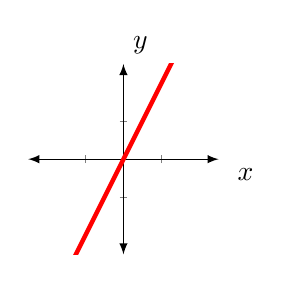
\begin{tikzpicture}[>=triangle 45,]
				\begin{axis}[
						    width = 4cm,
					               height = 4cm,
						    xmin=-2,xmax=2,
						    ymin=-2,ymax=2,
						    grid=none,
						    grid style={line width=.15pt, draw=gray!20},
						    major grid style={line width=.3pt,draw=gray!75},
						    axis lines=middle,
						    minor tick num=1,
						    enlargelimits={abs=0.5},
						    axis line style={latex-latex},
						    ticklabel style={font=\tiny,fill=white},
						    ticks=none,
						    xlabel={\,\,$x$},
						    ylabel={$y$},
						    xlabel style={below right},
						    ylabel style={above right},
						]
						\addplot+[<->, red, ultra thick,samples=100, mark=none] {2*x};
				\end{axis}
			\end{tikzpicture}
	\end{center}
\end{minipage}
&
\begin{minipage}[t]{0.2\linewidth}
	\begin{center}
	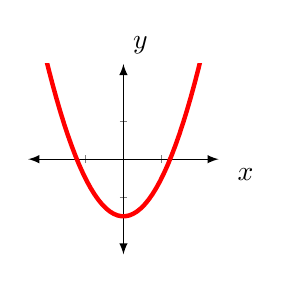
\begin{tikzpicture}[>=triangle 45,]
				\begin{axis}[
						    width = 4cm,
					               height = 4cm,
						    xmin=-2,xmax=2,
						    ymin=-2,ymax=2,
						    grid=none,
						    grid style={line width=.15pt, draw=gray!20},
						    major grid style={line width=.3pt,draw=gray!75},
						    axis lines=middle,
						    minor tick num=1,
						    enlargelimits={abs=0.5},
						    axis line style={latex-latex},
						    ticklabel style={font=\tiny,fill=white},
						    ticks=none,
						    xlabel={\,\,$x$},
						    ylabel={$y$},
						    xlabel style={below right},
						    ylabel style={above right},
						]
						\addplot+[<->, red, ultra thick,samples=100, mark=none] {x^2-1.5};
				\end{axis}
			\end{tikzpicture}
	\end{center}
\end{minipage}
&
\begin{minipage}[t]{0.2\linewidth}
	\begin{center}
	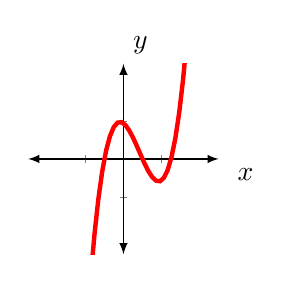
\begin{tikzpicture}[>=triangle 45,]
				\begin{axis}[
						    width = 4cm,
					               height = 4cm,
						    xmin=-2,xmax=2,
						    ymin=-2,ymax=2,
						    grid=none,
						    grid style={line width=.15pt, draw=gray!20},
						    major grid style={line width=.3pt,draw=gray!75},
						    axis lines=middle,
						    minor tick num=1,
						    enlargelimits={abs=0.5},
						    axis line style={latex-latex},
						    ticklabel style={font=\tiny,fill=white},
						    ticks=none,
						    xlabel={\,\,$x$},
						    ylabel={$y$},
						    xlabel style={below right},
						    ylabel style={above right},
						]
						\addplot+[<->, red, ultra thick,samples=100, mark=none] {3* (x-0.5)*(x+0.5)*(x-1.25)};
				\end{axis}
			\end{tikzpicture}
	\end{center}
\end{minipage}
&
\begin{minipage}[t]{0.2\linewidth}
	\begin{center}
	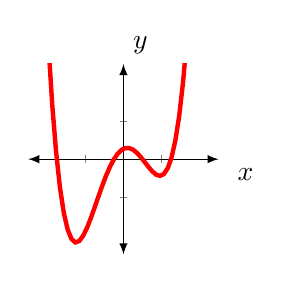
\begin{tikzpicture}[>=triangle 45,]
				\begin{axis}[
						    width = 4cm,
					               height = 4cm,
						    xmin=-2,xmax=2,
						    ymin=-2,ymax=2,
						    grid=none,
						    grid style={line width=.15pt, draw=gray!20},
						    major grid style={line width=.3pt,draw=gray!75},
						    axis lines=middle,
						    minor tick num=1,
						    enlargelimits={abs=0.5},
						    axis line style={latex-latex},
						    ticklabel style={font=\tiny,fill=white},
						    ticks=none,
						    xlabel={\,\,$x$},
						    ylabel={$y$},
						    xlabel style={below right},
						    ylabel style={above right},
						]
						\addplot+[<->, red, ultra thick,samples=100, mark=none] {(x+1.75)*(x+0.25)*(x-0.5)*(x-1.25)};
				\end{axis}
			\end{tikzpicture}
	\end{center}
\end{minipage}
&
\begin{minipage}[t]{0.2\linewidth}
	\begin{center}
	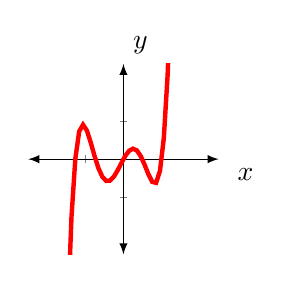
\begin{tikzpicture}[>=triangle 45,]
				\begin{axis}[
						    width = 4cm,
					               height = 4cm,
						    xmin=-2,xmax=2,
						    ymin=-2,ymax=2,
						    grid=none,
						    grid style={line width=.15pt, draw=gray!20},
						    major grid style={line width=.3pt,draw=gray!75},
						    axis lines=middle,
						    minor tick num=1,
						    enlargelimits={abs=0.5},
						    axis line style={latex-latex},
						    ticklabel style={font=\tiny,fill=white},
						    ticks=none,
						    xlabel={\,\,$x$},
						    ylabel={$y$},
						    xlabel style={below right},
						    ylabel style={above right},
						]
						\addplot+[<->, red, ultra thick,samples=100, mark=none,restrict y to domain=-100:100] {4*(x^5+0.5*x^4-1.57*x^3-0.4*x^2+0.46*x)};
				\end{axis}
			\end{tikzpicture}
	\end{center}
\end{minipage}
\\
\hline
\end{tabular}

\begin{definition}
\textbf{End behavior} is a description of the values of a function ($y$-values) as $x$ approaches positive infinity ($x \longrightarrow \infty$) or negative infinity ($x\longrightarrow \infty$).
\end{definition}

\begin{center}
\begin{tabular}[t]{|c|c|c|}
\hline
\multicolumn{3}{|c|}{}\\
\multicolumn{3}{|c|}{\textbf{Polynomial End Behavior}}\\
\hline
&&\\
$\mathbf{P(x)\,} \textbf{ has..} $ &\textbf{Odd Degree} & \textbf{Even Degree}\\
\hline
Leading&&\\
Coefficient &&\\
$a>0$ &&\\
&
\begin{minipage}[t]{0.2\linewidth}
	\vspace{-1.5cm}
	\begin{center}
	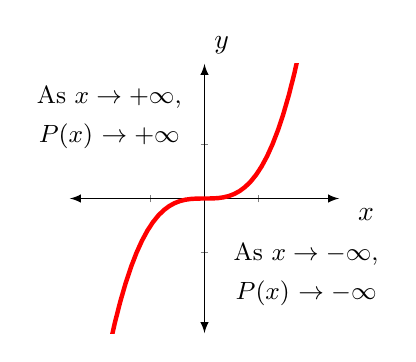
\begin{tikzpicture}[>=triangle 45,]
				\begin{axis}[
						    width = 5cm,
					               height = 5cm,
						    xmin=-2,xmax=2,
						    ymin=-2,ymax=2,
						    grid=none,
						    grid style={line width=.15pt, draw=gray!20},
						    major grid style={line width=.3pt,draw=gray!75},
						    axis lines=middle,
						    minor tick num=1,
						    enlargelimits={abs=0.5},
						    axis line style={latex-latex},
						    ticklabel style={font=\tiny,fill=white},
						    ticks=none,
						    xlabel={\,\,$x$},
						    ylabel={$y$},
						    xlabel style={below right},
						    ylabel style={above right},
						]
						\addplot+[<->, red, ultra thick,samples=100, mark=none] {0.5*x^3};
				\end{axis}
				\draw (0.5,3) node{\small As $ x\rightarrow +\infty$,};
				\draw (0.5,2.5) node{\small$P(x)$ $\rightarrow +\infty$};
				\draw (3,1) node{\small As $ x\rightarrow -\infty$,};
				\draw (3,0.5) node{\small$P(x)$ $\rightarrow -\infty$};
			\end{tikzpicture}	
	\end{center}
\end{minipage}
\hspace{1cm}
&
\begin{minipage}[t]{0.2\linewidth}
	\vspace{-1.5cm}
	\begin{center}
	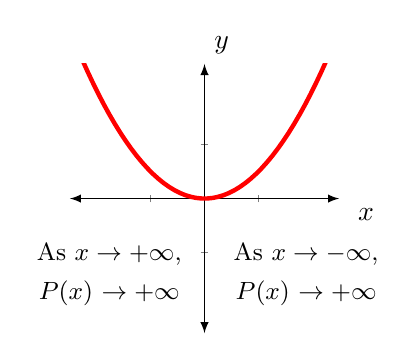
\begin{tikzpicture}[>=triangle 45,]
				\begin{axis}[
						    width = 5cm,
					               height = 5cm,
						    xmin=-2,xmax=2,
						    ymin=-2,ymax=2,
						    grid=none,
						    grid style={line width=.15pt, draw=gray!20},
						    major grid style={line width=.3pt,draw=gray!75},
						    axis lines=middle,
						    minor tick num=1,
						    enlargelimits={abs=0.5},
						    axis line style={latex-latex},
						    ticklabel style={font=\tiny,fill=white},
						    ticks=none,
						    xlabel={\,\,$x$},
						    ylabel={$y$},
						    xlabel style={below right},
						    ylabel style={above right},
						]
						\addplot+[<->, red, ultra thick,samples=100, mark=none] {0.5*x^2};
				\end{axis}
				\draw (0.5,1) node{\small As $ x\rightarrow +\infty$,};
				\draw (0.5,0.5) node{\small$P(x)$ $\rightarrow +\infty$};
				\draw (3,1) node{\small As $ x\rightarrow -\infty$,};
				\draw (3,0.5) node{\small$P(x)$ $\rightarrow +\infty$};
			\end{tikzpicture}	
	\end{center}
\end{minipage}
\hspace{1cm}
\\
\hline
Leading&&\\
Coefficient &&\\
$a<0$ &&\\
&
\begin{minipage}[t]{0.2\linewidth}
	\vspace{-1.5cm}
	\begin{center}
	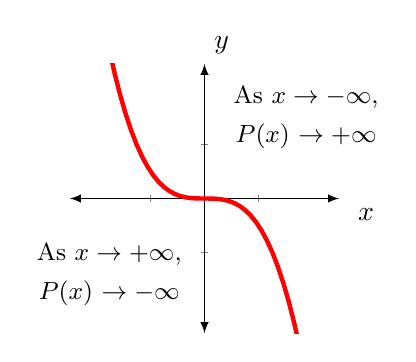
\begin{tikzpicture}[>=triangle 45,]
				\begin{axis}[
						    width = 5cm,
					               height = 5cm,
						    xmin=-2,xmax=2,
						    ymin=-2,ymax=2,
						    grid=none,
						    grid style={line width=.15pt, draw=gray!20},
						    major grid style={line width=.3pt,draw=gray!75},
						    axis lines=middle,
						    minor tick num=1,
						    enlargelimits={abs=0.5},
						    axis line style={latex-latex},
						    ticklabel style={font=\tiny,fill=white},
						    ticks=none,
						    xlabel={\,\,$x$},
						    ylabel={$y$},
						    xlabel style={below right},
						    ylabel style={above right},
						]
						\addplot+[<->, red, ultra thick,samples=100, mark=none] {-0.5*x^3};
				\end{axis}
				\draw (0.5,1) node{\small As $ x\rightarrow +\infty$,};
				\draw (0.5,0.5) node{\small$P(x)$ $\rightarrow -\infty$};
				\draw (3,3) node{\small As $ x\rightarrow -\infty$,};
				\draw (3,2.5) node{\small$P(x)$ $\rightarrow +\infty$};
			\end{tikzpicture}	
	\end{center}
\end{minipage}
\hspace{1cm}
&
\begin{minipage}[t]{0.2\linewidth}
	\vspace{-1.5cm}
	\begin{center}
	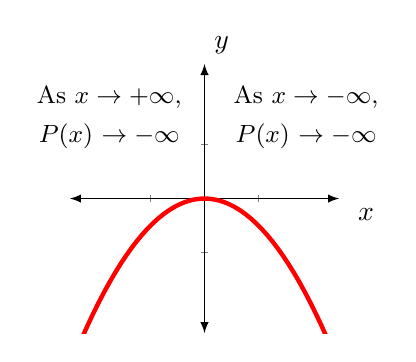
\begin{tikzpicture}[>=triangle 45,]
				\begin{axis}[
						    width = 5cm,
					               height = 5cm,
						    xmin=-2,xmax=2,
						    ymin=-2,ymax=2,
						    grid=none,
						    grid style={line width=.15pt, draw=gray!20},
						    major grid style={line width=.3pt,draw=gray!75},
						    axis lines=middle,
						    minor tick num=1,
						    enlargelimits={abs=0.5},
						    axis line style={latex-latex},
						    ticklabel style={font=\tiny,fill=white},
						    ticks=none,
						    xlabel={\,\,$x$},
						    ylabel={$y$},
						    xlabel style={below right},
						    ylabel style={above right},
						]
						\addplot+[<->, red, ultra thick,samples=100, mark=none] {-0.5*x^2};
				\end{axis}
				\draw (0.5,3) node{\small As $ x\rightarrow +\infty$,};
				\draw (0.5,2.5) node{\small$P(x)$ $\rightarrow -\infty$};
				\draw (3,3) node{\small As $ x\rightarrow -\infty$,};
				\draw (3,2.5) node{\small$P(x)$ $\rightarrow -\infty$};
			\end{tikzpicture}	
	\end{center}
\end{minipage}
\hspace{1cm}
\\
\hline
\end{tabular}
\end{center}

\begin{example}
Identify the leading coefficient, degree and end behavior.
\end{example}

\begin{minipage}[t]{0.45\linewidth}
(a) $P(x)=-4x^3-3x^2+5x+6$\\

\underline{Degree:}\\

\underline{Leading Coefficient}\\

\underline{End Behavior:} As $x\longrightarrow +\infty$\\


 \hspace{2.35cm }As $x\longrightarrow -\infty$
\end{minipage}
\hfill
\begin{minipage}[t]{0.45\linewidth}
(b) $R(x)=x^6-7x^5+x^3-2$\\

\underline{Degree:}\\

\underline{Leading Coefficient}\\

\underline{End Behavior:} As $x\longrightarrow +\infty$\\


 \hspace{2.35cm }As $x\longrightarrow -\infty$
\end{minipage}


%%%%%%%%%%%%%%%%%%%%%%%%%%%%%%%%%%%%%
%%%%%%%%%%%%%%%%%%%%%%%%%%%%%%%%%%%%%
 \newpage
%%%%%%%%%%%%%%%%%%%%%%%%%%%%%%%%%%%%%
%%%%%%%%%%%%%%%%%%%%%%%%%%%%%%%%%%%%%

\begin{example}
Identify whether the function graphed has an odd or even degree and a positive or negative leading coefficient.
\end{example}



\begin{minipage}[t]{0.45\linewidth}
(a)
\vspace{-1cm}
	\begin{center}
	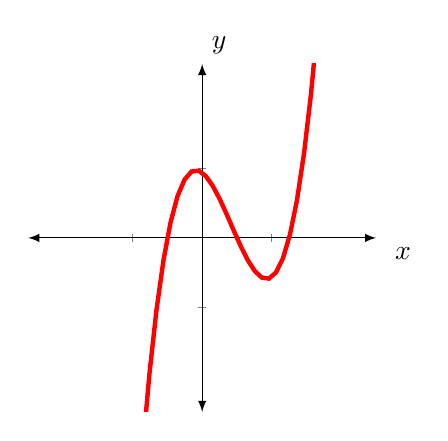
\begin{tikzpicture}[>=triangle 45,]
				\begin{axis}[
						    width = 6cm,
					               height = 6cm,
						    xmin=-2,xmax=2,
						    ymin=-2,ymax=2,
						    grid=none,
						    grid style={line width=.15pt, draw=gray!20},
						    major grid style={line width=.3pt,draw=gray!75},
						    axis lines=middle,
						    minor tick num=1,
						    enlargelimits={abs=0.5},
						    axis line style={latex-latex},
						    ticklabel style={font=\tiny,fill=white},
						    ticks=none,
						    xlabel={\,\,$x$},
						    ylabel={$y$},
						    xlabel style={below right},
						    ylabel style={above right},
						]
						\addplot+[<->, red, ultra thick,samples=100, mark=none, restrict y to domain=-25:25] {3* (x-0.5)*(x+0.5)*(x-1.25)};
				\end{axis}
			\end{tikzpicture}
	\end{center}
	\underline{Degree:}\\
	
	\underline{Leading Coefficient:}\\
	
	(c)
\vspace{-1cm}
	\begin{center}
	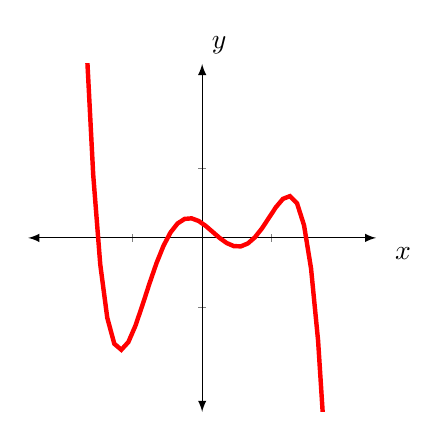
\begin{tikzpicture}[>=triangle 45,]
				\begin{axis}[
						    width = 6cm,
					               height = 6cm,
						    xmin=-2,xmax=2,
						    ymin=-2,ymax=2,
						    grid=none,
						    grid style={line width=.15pt, draw=gray!20},
						    major grid style={line width=.3pt,draw=gray!75},
						    axis lines=middle,
						    minor tick num=1,
						    enlargelimits={abs=0.5},
						    axis line style={latex-latex},
						    ticklabel style={font=\tiny,fill=white},
						    ticks=none,
						    xlabel={\,\,$x$},
						    ylabel={$y$},
						    xlabel style={below right},
						    ylabel style={above right},
						]
						\addplot+[<->, red, ultra thick,samples=100, mark=none, restrict y to domain=-25:25] {-1* (x-1.5)*(x+1.5)*(x-0.25)*(x-0.75)*(x+0.5)};
				\end{axis}
			\end{tikzpicture}
	\end{center}
	\underline{Degree:}\\
	
	\underline{Leading Coefficient:}\\
\end{minipage}
\hfill
\begin{minipage}[t]{0.45\linewidth}
(b)
\vspace{-1cm}
	\begin{center}
	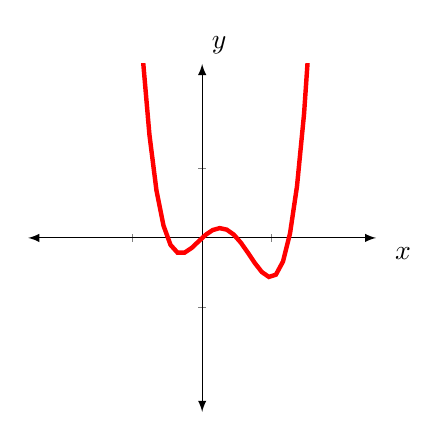
\begin{tikzpicture}[>=triangle 45,]
				\begin{axis}[
						    width = 6cm,
					               height = 6cm,
						    xmin=-2,xmax=2,
						    ymin=-2,ymax=2,
						    grid=none,
						    grid style={line width=.15pt, draw=gray!20},
						    major grid style={line width=.3pt,draw=gray!75},
						    axis lines=middle,
						    minor tick num=1,
						    enlargelimits={abs=0.5},
						    axis line style={latex-latex},
						    ticklabel style={font=\tiny,fill=white},
						    ticks=none,
						    xlabel={\,\,$x$},
						    ylabel={$y$},
						    xlabel style={below right},
						    ylabel style={above right},
						]
						\addplot+[<->, red, ultra thick,samples=100, mark=none, restrict y to domain=-25:25] {3* (x-0.5)*(x+0.5)*(x-1.25)*x};
				\end{axis}
			\end{tikzpicture}
	\end{center}
	\underline{Degree:}\\
	
	\underline{Leading Coefficient:}\\
	
	(d)
	\vspace{-1cm}
	\begin{center}
	\begin{tikzpicture}[>=triangle 45,]
				\begin{axis}[
						    width = 6cm,
					               height = 6cm,
						    xmin=-2,xmax=2,
						    ymin=-2,ymax=2,
						    grid=none,
						    grid style={line width=.15pt, draw=gray!20},
						    major grid style={line width=.3pt,draw=gray!75},
						    axis lines=middle,
						    minor tick num=1,
						    enlargelimits={abs=0.5},
						    axis line style={latex-latex},
						    ticklabel style={font=\tiny,fill=white},
						    ticks=none,
						    xlabel={\,\,$x$},
						    ylabel={$y$},
						    xlabel style={below right},
						    ylabel style={above right},
						]
						\addplot+[<->, red, ultra thick,samples=100, mark=none, restrict y to domain=-25:25] {-2*x^2-2*x-1};
				\end{axis}
			\end{tikzpicture}
	\end{center}
	\underline{Degree:}\\
	
	\underline{Leading Coefficient:}\\
\end{minipage}

\begin{youtry}
Identify whether the function graphed has an odd or even degree and a positive or negative leading coefficient.
\end{youtry}

\begin{minipage}[t]{0.45\linewidth}
(a)
\vspace{-1cm}
	\begin{center}
	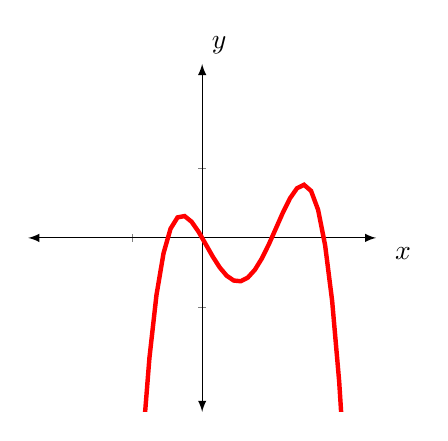
\begin{tikzpicture}[>=triangle 45,]
				\begin{axis}[
						    width = 6cm,
					               height = 6cm,
						    xmin=-2,xmax=2,
						    ymin=-2,ymax=2,
						    grid=none,
						    grid style={line width=.15pt, draw=gray!20},
						    major grid style={line width=.3pt,draw=gray!75},
						    axis lines=middle,
						    minor tick num=1,
						    enlargelimits={abs=0.5},
						    axis line style={latex-latex},
						    ticklabel style={font=\tiny,fill=white},
						    ticks=none,
						    xlabel={\,\,$x$},
						    ylabel={$y$},
						    xlabel style={below right},
						    ylabel style={above right},
						]
						\addplot+[<->, red, ultra thick,samples=100, mark=none, restrict y to domain=-25:25] {-2*(x-1.75)*(x-1)*(x)*(x+0.5)};
				\end{axis}
			\end{tikzpicture}
	\end{center}
	\underline{Degree:}\\
	
	\underline{Leading Coefficient:}\\
\end{minipage}
\hfill
\begin{minipage}[t]{0.45\linewidth}
(b)
\vspace{-1cm}
	\begin{center}
	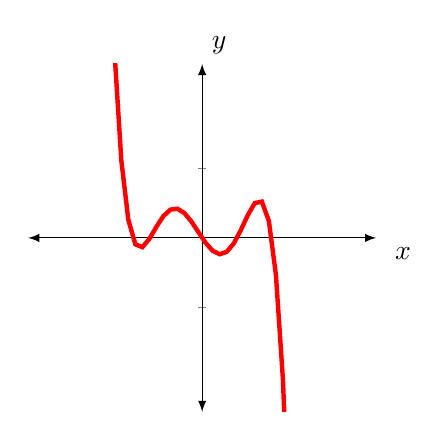
\begin{tikzpicture}[>=triangle 45,]
				\begin{axis}[
						    width = 6cm,
					               height = 6cm,
						    xmin=-2,xmax=2,
						    ymin=-2,ymax=2,
						    grid=none,
						    grid style={line width=.15pt, draw=gray!20},
						    major grid style={line width=.3pt,draw=gray!75},
						    axis lines=middle,
						    minor tick num=1,
						    enlargelimits={abs=0.5},
						    axis line style={latex-latex},
						    ticklabel style={font=\tiny,fill=white},
						    ticks=none,
						    xlabel={\,\,$x$},
						    ylabel={$y$},
						    xlabel style={below right},
						    ylabel style={above right},
						]
						\addplot+[<->, red, ultra thick,samples=100, mark=none, restrict y to domain=-25:25] {-4*(x-1)*(x-0.5)*(x+0.75)*x*(x+1)};
				\end{axis}
			\end{tikzpicture}
	\end{center}
	\underline{Degree:}\\
	
	\underline{Leading Coefficient:}\\
\end{minipage}

\vfill
 \noindent\fbox{\large\textbf{6.7 Homework (day 1)}: page 457 \, 2-9, 15-21 odd \small }
%%%%%%%%%%%%%%%%%%%%%%%%%%%%%%%%%%%%%
%%%%%%%%%%%%%%%%%%%%%%%%%%%%%%%%%%%%%
 \newpage
%%%%%%%%%%%%%%%%%%%%%%%%%%%%%%%%%%%%%
%%%%%%%%%%%%%%%%%%%%%%%%%%%%%%%%%%%%%

\noindent\Large\textbf{6.7 Investigating Graphs of Polynomial Functions (day 2)}\\

 \indent\hfill\small\noindent \textbf{Objective}: Identify and use maxima and minima of polynomial functions to solve problems. \normalsize\\

\vspace{-0.75cm}

\begin{center}
\begin{tabular}[t]{|l|}
\hline
\\
\multicolumn{1}{|c|}{\textbf{Steps for Graphing a Polynomial Function}}\\
\hline
\\
1. Find all zeros (x-intercepts) and y-intercepts of the function.\\
\hline
\\
2. Plot the $x$- and $y$-intercept.\\
\hline
\\
3. Make a table for several $x$-values that lie between the real zeros.\\
\hline
\\
4. Plot the points from your table.\\
\hline
\\
5. Determine end behavior.\\
\hline
\\
6. Sketch the graph.\\
\hline
\end{tabular}
\end{center}

\begin{example}
Graph the function.
\end{example}
$f(x)=x^3+3x^2-6x-8$


\vspace{-1.5cm}

\begin{flushright}
	 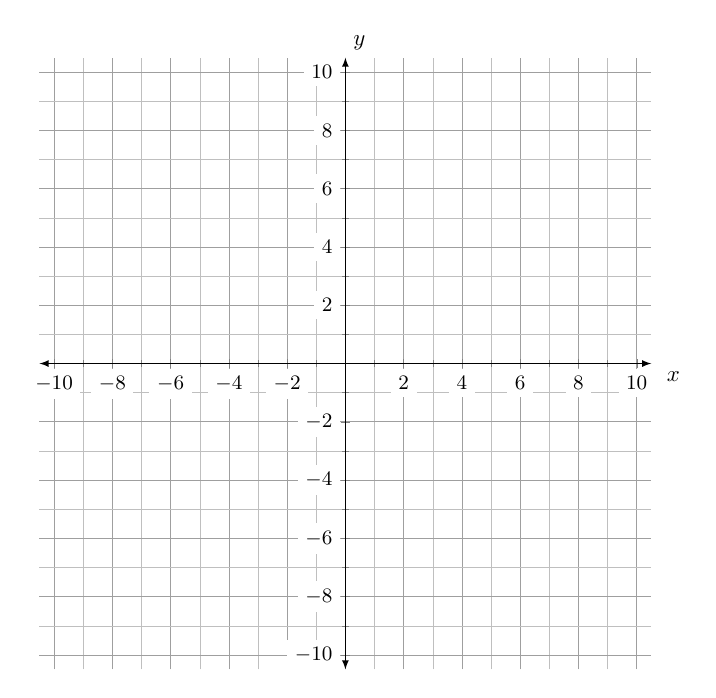
\begin{tikzpicture}[>=latex,scale=0.825]
			\begin{axis}[
					    width =11cm,
				               height=11cm,
					    xmin=-10,xmax=10,
					    ymin=-10,ymax=10,
					    grid=both,
					     grid style={line width=.2pt, draw=gray!50},
					    major grid style={line width=.3pt,draw=gray!75},
					    axis lines=middle,
					    minor tick num=1,
					    enlargelimits={abs=0.5},
					    axis line style={latex-latex},
					    ticklabel style={font=\small,fill=white},
					    xlabel={\,\,$x$},
					    ylabel={$y$},
					    xlabel style={below right},
					    ylabel style={above right},
					]
			\end{axis}
			%\draw[color=blue,thick] plot (\x,\x*\x);
	\end{tikzpicture}
\end{flushright}

\vfill

\vspace{-0.25cm}

\begin{example}
Graph the function.
\end{example}
$f(x)=-x^3+2x^2+5x-6$

\vspace{-1.5cm}

\begin{flushright}
	 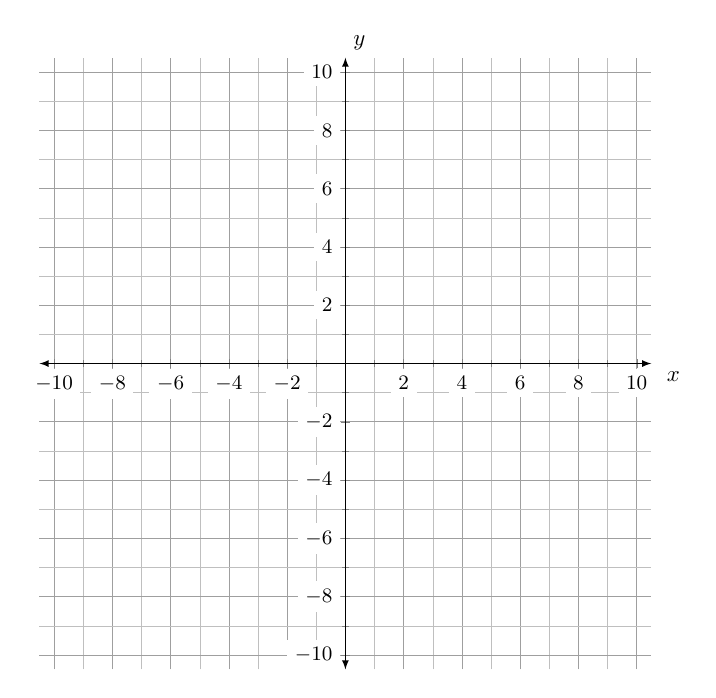
\begin{tikzpicture}[>=latex,scale=0.825]
			\begin{axis}[
					    width =11cm,
				               height=11cm,
					    xmin=-10,xmax=10,
					    ymin=-10,ymax=10,
					    grid=both,
					    grid style={line width=.2pt, draw=gray!50},
					    major grid style={line width=.3pt,draw=gray!75},
					    axis lines=middle,
					    minor tick num=1,
					    enlargelimits={abs=0.5},
					    axis line style={latex-latex},
					    ticklabel style={font=\small,fill=white},
					    xlabel={\,\,$x$},
					    ylabel={$y$},
					    xlabel style={below right},
					    ylabel style={above right},
					]
			\end{axis}
			%\draw[color=blue,thick] plot (\x,\x*\x);
	\end{tikzpicture}
\end{flushright}

%%%%%%%%%%%%%%%%%%%%%%%%%%%%%%%%%%%%%
%%%%%%%%%%%%%%%%%%%%%%%%%%%%%%%%%%%%%
 \newpage
%%%%%%%%%%%%%%%%%%%%%%%%%%%%%%%%%%%%%
%%%%%%%%%%%%%%%%%%%%%%%%%%%%%%%%%%%%%

\begin{definition}
For a function $f(x)$, $f(a)$ is a \textbf{local maximum} if there is an interval around a such that $f(x)<f(a)$ for every $x$-value in the interval except $a$.
\end{definition}

\begin{definition}
\,\,For a function $f(x)$, $f(a)$ is a \textbf{local minimum} if there is an interval around a such that \,\,$f(x)>f(a)$ for every $x$-value in the interval except $a$.
\end{definition}

\vspace{0.5cm}

\noindent\large\textbf{Determine Maxima and Minima with a calculator}\normalsize\\

\textbf{Step 1:} Type equations into \tcbox[size=small, on line]{$Y=$} and press  \tcbox[size=small, on line]{GRAPH}.\\

\vspace{-0.5cm}

\begin{center}
\begin{minipage}[t]{0.85\linewidth}
The graph appears to have one local maximum or minimum.\\
\end{minipage}
\end{center}

\textbf{Step 2:} Find the maximum.\\

\vspace{-0.5cm}

\begin{center}
\begin{minipage}[t]{0.85\linewidth}
Press \tcbox[size=small, on line]{2nd} \tcbox[size=small, on line]{TRACE} to access the \texttt{CALC} menu. Choose \textbf{4: maximum}. Arrow to the left of maximum and press \tcbox[size=small, on line]{ENTER}, next arrow to the right of the maximum and press \tcbox[size=small, on line]{ENTER}.\\
\end{minipage}
\end{center}

\textbf{Step 3:} Find the minimum.\\

\vspace{-0.5cm}

\begin{center}
\begin{minipage}[t]{0.85\linewidth}
Press \tcbox[size=small, on line]{2nd} \tcbox[size=small, on line]{TRACE} to access the \texttt{CALC} menu. Choose \textbf{3: minimum}. Arrow to the left of minimum and press \tcbox[size=small, on line]{ENTER}, next arrow to the right of the minimum and press \tcbox[size=small, on line]{ENTER}.\\
\end{minipage}
\end{center}


\begin{example}
Graph the function on a calculator, and estimate the local \textbf{maxima} and \textbf{minima}. 
\end{example}

\begin{minipage}[t]{0.45\linewidth}
(a) $g(x)=2x^3-12x+6$
\end{minipage}
\hfill
\begin{minipage}[t]{0.45\linewidth}
(b) $f(x)=x^3-2x-3$
\end{minipage}

\vfill

\begin{example}
A welder plans to construct an open box from an 18.5 ft by 24.5 ft sheet of metal by cutting squares from the corners and folding up the sides. Find the maximum volume of the box and the corresponding dimensions.
\end{example}


\vfill

 \noindent\fbox{\large\textbf{6.7 Homework (day 2)}: page 457 \, 10-14 all, 23, 25 \small }

%%%%%%%%%%%%%%%%%%%%%%%%%%%%%%%%%%%%%
%%%%%%%%%%%%%%%%%%%%%%%%%%%%%%%%%%%%%
 \newpage
%%%%%%%%%%%%%%%%%%%%%%%%%%%%%%%%%%%%%
%%%%%%%%%%%%%%%%%%%%%%%%%%%%%%%%%%%%%

\noindent\Large\textbf{6.7 Investigating Graphs of Polynomial Functions (day 3)}\\\large

\noindent Sketch the polynomial function with the given properties.\normalsize\\

%%%% #1
\begin{minipage}[t]{0.45\linewidth}
\small
	\begin{minipage}[t]{0.45\linewidth}
		\underline{Leading Coefficient}: -2\\
		
		\underline{Degree}: 6 \\
		
		\underline{y-intercept}: 2 \\
		
	\end{minipage}
	\begin{minipage}[t]{0.45\linewidth}
		\begin{tabular}[t]{c|c}
			Roots & Multiplicity\\
			\hline
			-6&1\\
			-2&2\\
			2&2\\
			4&1\\
		\end{tabular}
	\end{minipage}
\normalsize
	\vspace{-0.5cm}
	\begin{center}
		 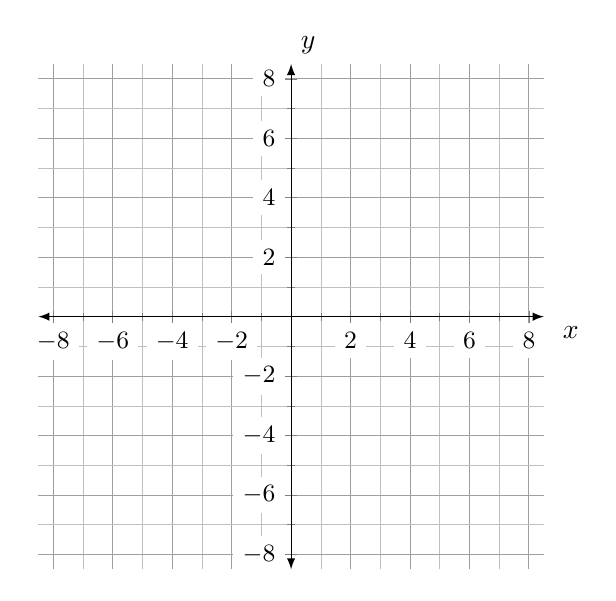
\begin{tikzpicture}[>=latex,scale=1]
				\begin{axis}[
						    width =8cm,
					               height=8cm,
						    xmin=-8,xmax=8,
						    ymin=-8,ymax=8,
						    grid=both,
						    grid style={line width=.2pt, draw=gray!50},
						    major grid style={line width=.3pt,draw=gray!75},
						    axis lines=middle,
						    minor tick num=1,
						    enlargelimits={abs=0.5},
						    axis line style={latex-latex},
						    ticklabel style={font=\small,fill=white},
						    xlabel={\,\,$x$},
						    ylabel={$y$},
						    xlabel style={below right},
						    ylabel style={above right},
						]
				\end{axis}
				%\draw[color=blue,thick] plot (\x,\x*\x);
		\end{tikzpicture}
	\end{center}
\end{minipage}
\hfill
%%%% #2
\begin{minipage}[t]{0.45\linewidth}
\small
	\begin{minipage}[t]{0.45\linewidth}
		\underline{Leading Coefficient}: -1\\
		
		\underline{Degree}: 5 \\
		
		\underline{y-intercept}: -5 \\
		
	\end{minipage}
	\begin{minipage}[t]{0.45\linewidth}
		\begin{tabular}[t]{c|c}
			Roots & Multiplicity\\
			\hline
			-7&2\\
			-2&3\\
		\end{tabular}
	\end{minipage}
\normalsize
	\vspace{-0.5cm}
	\begin{center}
		 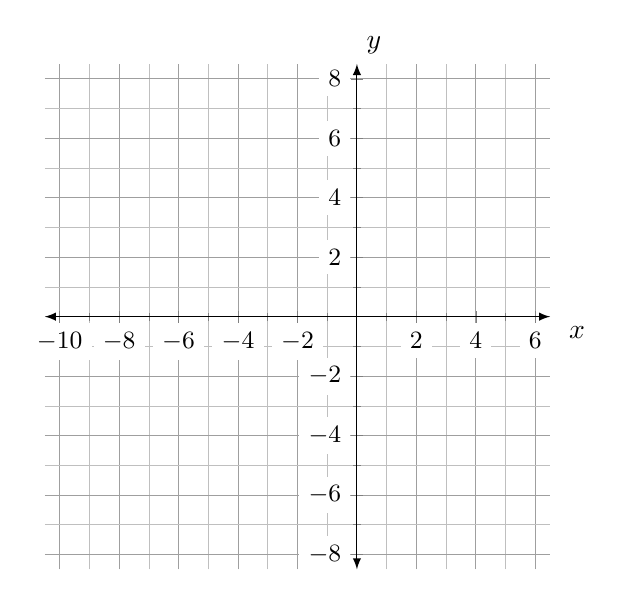
\begin{tikzpicture}[>=latex,scale=1]
				\begin{axis}[
						    width =8cm,
					               height=8cm,
						    xmin=-10,xmax=6,
						    ymin=-8,ymax=8,
						    grid=both,
						    grid style={line width=.2pt, draw=gray!50},
						    major grid style={line width=.3pt,draw=gray!75},
						    axis lines=middle,
						    minor tick num=1,
						    enlargelimits={abs=0.5},
						    axis line style={latex-latex},
						    ticklabel style={font=\small,fill=white},
						    xlabel={\,\,$x$},
						    ylabel={$y$},
						    xlabel style={below right},
						    ylabel style={above right},
						]
				\end{axis}
				%\draw[color=blue,thick] plot (\x,\x*\x);
		\end{tikzpicture}
	\end{center}
\end{minipage}
%%%%%%%%%%%%%%%NEW LINE%%%%%%%%%%%%%%%%%%%%%%
\vfill

%%%%%% #3
\begin{minipage}[t]{0.45\linewidth}
\small
	\begin{minipage}[t]{0.45\linewidth}
		\underline{Leading Coefficient}: 5\\
		
		\underline{Degree}: 3 \\
		
		\underline{y-intercept}: -3 \\
		
	\end{minipage}
	\begin{minipage}[t]{0.45\linewidth}
		\begin{tabular}[t]{c|c}
			Roots & Multiplicity\\
			\hline
			-4&1\\
			-1&1\\
			2&1\\
		\end{tabular}
	\end{minipage}
\normalsize
	\vspace{-0.5cm}
	\begin{center}
		 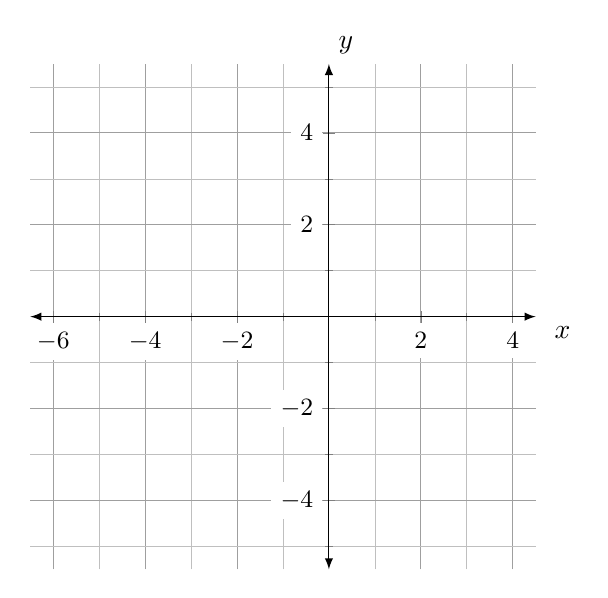
\begin{tikzpicture}[>=latex,scale=1]
				\begin{axis}[
						    width =8cm,
					               height=8cm,
						    xmin=-6,xmax=4,
						    ymin=-5,ymax=5,
						    grid=both,
						    grid style={line width=.2pt, draw=gray!50},
						    major grid style={line width=.3pt,draw=gray!75},
						    axis lines=middle,
						    minor tick num=1,
						    enlargelimits={abs=0.5},
						    axis line style={latex-latex},
						    ticklabel style={font=\small,fill=white},
						    xlabel={\,\,$x$},
						    ylabel={$y$},
						    xlabel style={below right},
						    ylabel style={above right},
						]
				\end{axis}
				%\draw[color=blue,thick] plot (\x,\x*\x);
		\end{tikzpicture}
	\end{center}
\end{minipage}
\hfill
%%%%% #4
\begin{minipage}[t]{0.45\linewidth}
\small
	\begin{minipage}[t]{0.45\linewidth}
		\underline{Leading Coefficient}: -1\\
		
		\underline{Degree}: 2 \\
		
		\underline{y-intercept}: -2 \\
		
	\end{minipage}
	\begin{minipage}[t]{0.45\linewidth}
		\begin{tabular}[t]{c|c}
			Roots & Multiplicity\\
			\hline
			\multicolumn{2}{c}{no real roots}
		\end{tabular}
	\end{minipage}
\normalsize
	\vspace{-0.5cm}
	\begin{center}
		 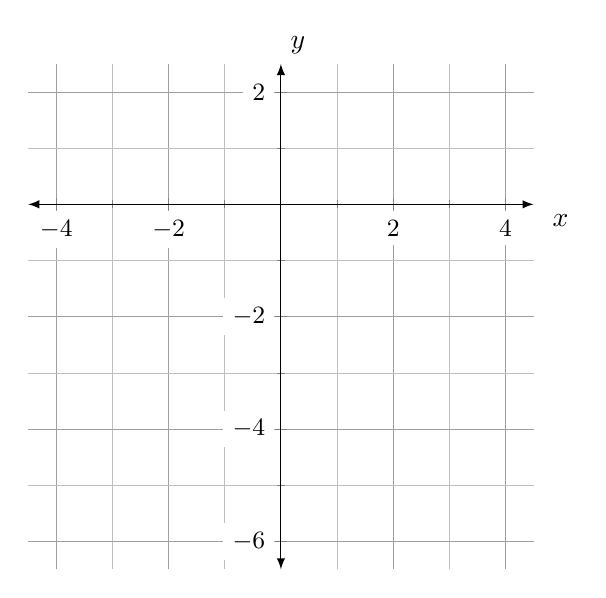
\begin{tikzpicture}[>=latex,scale=1]
				\begin{axis}[
						    width =8cm,
					               height=8cm,
						    xmin=-4,xmax=4,
						    ymin=-6,ymax=2,
						    grid=both,
						    grid style={line width=.2pt, draw=gray!50},
						    major grid style={line width=.3pt,draw=gray!75},
						    axis lines=middle,
						    minor tick num=1,
						    enlargelimits={abs=0.5},
						    axis line style={latex-latex},
						    ticklabel style={font=\small,fill=white},
						    xlabel={\,\,$x$},
						    ylabel={$y$},
						    xlabel style={below right},
						    ylabel style={above right},
						]
				\end{axis}
				%\draw[color=blue,thick] plot (\x,\x*\x);
		\end{tikzpicture}
	\end{center}
\end{minipage}
%%%%%%%%%%%%NEW LINE%%%%%%%%%%%%%%%%%%%%%%%%%
\vfill

%%%%%%%%%%%%%%%%%%%%%%%%%%%%%%%%%%%%%
%%%%%%%%%%%%%%%%%%%%%%%%%%%%%%%%%%%%%
 \newpage
%%%%%%%%%%%%%%%%%%%%%%%%%%%%%%%%%%%%%
%%%%%%%%%%%%%%%%%%%%%%%%%%%%%%%%%%%%%


\noindent Sketch the polynomial function with the given properties.\normalsize\\


%%%%% #5
\begin{minipage}[t]{0.45\linewidth}
\small
	\begin{minipage}[t]{0.45\linewidth}
		\underline{Leading Coefficient}: 1\\
		
		\underline{Degree}: 7 \\
		
		\underline{y-intercept}: 0 \\
		
	\end{minipage}
	\begin{minipage}[t]{0.45\linewidth}
		\begin{tabular}[t]{c|c}
			Roots & Multiplicity\\
			\hline
			-7&3\\
			-2&2\\
			0&2\\

		\end{tabular}
	\end{minipage}
\normalsize
	\vspace{-0.5cm}
	\begin{center}
		 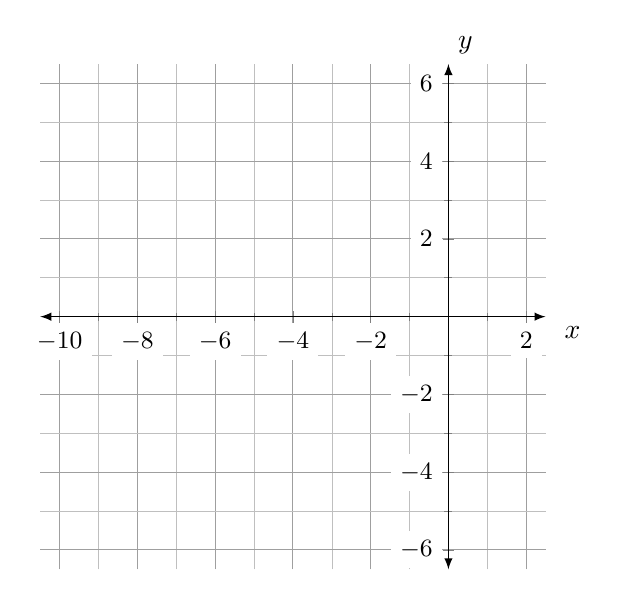
\begin{tikzpicture}[>=latex,scale=1]
				\begin{axis}[
						    width =8cm,
					               height=8cm,
						    xmin=-10,xmax=2,
						    ymin=-6,ymax=6,
						    grid=both,
						    grid style={line width=.2pt, draw=gray!50},
						    major grid style={line width=.3pt,draw=gray!75},
						    axis lines=middle,
						    minor tick num=1,
						    enlargelimits={abs=0.5},
						    axis line style={latex-latex},
						    ticklabel style={font=\small,fill=white},
						    xlabel={\,\,$x$},
						    ylabel={$y$},
						    xlabel style={below right},
						    ylabel style={above right},
						]
				\end{axis}
				%\draw[color=blue,thick] plot (\x,\x*\x);
		\end{tikzpicture}
	\end{center}
\end{minipage}
\hfill
%%%%% #6
\begin{minipage}[t]{0.45\linewidth}
\small
	\begin{minipage}[t]{0.45\linewidth}
		\underline{Leading Coefficient}: 1\\
		
		\underline{Degree}: 5 \\
		
		\underline{y-intercept}: -1 \\
		
	\end{minipage}
	\begin{minipage}[t]{0.45\linewidth}
		\begin{tabular}[t]{c|c}
			Roots & Multiplicity\\
			\hline
			-6&1\\
			-1&3\\
			4&1\\
		\end{tabular}
	\end{minipage}
\normalsize
	\vspace{-0.5cm}
	\begin{center}
		 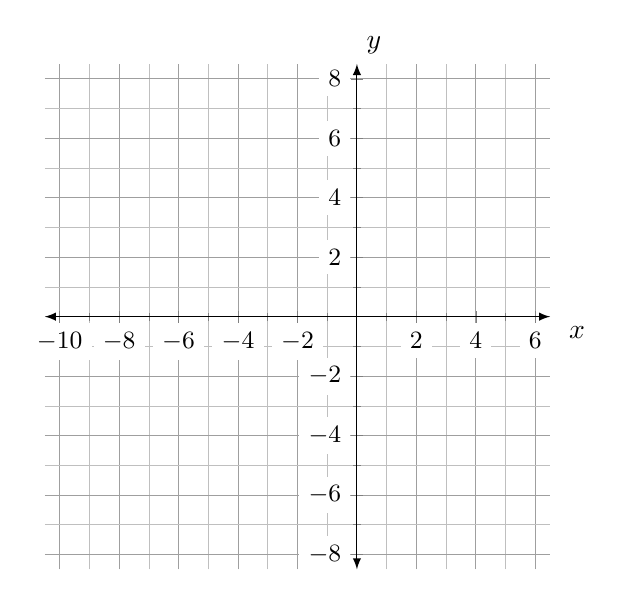
\begin{tikzpicture}[>=latex,scale=1]
				\begin{axis}[
						    width =8cm,
					               height=8cm,
						    xmin=-10,xmax=6,
						    ymin=-8,ymax=8,
						    grid=both,
						    grid style={line width=.2pt, draw=gray!50},
						    major grid style={line width=.3pt,draw=gray!75},
						    axis lines=middle,
						    minor tick num=1,
						    enlargelimits={abs=0.5},
						    axis line style={latex-latex},
						    ticklabel style={font=\small,fill=white},
						    xlabel={\,\,$x$},
						    ylabel={$y$},
						    xlabel style={below right},
						    ylabel style={above right},
						]
				\end{axis}
				%\draw[color=blue,thick] plot (\x,\x*\x);
		\end{tikzpicture}
	\end{center}
\end{minipage}
%%%%%%%%%%%%%%%NEW LINE%%%%%%%%%%%%%%%%%%%%%%
\vfill

%%%%% # 7
\begin{minipage}[t]{0.45\linewidth}
\small
	\begin{minipage}[t]{0.45\linewidth}
		\underline{Leading Coefficient}: 2\\
		
		\underline{Degree}: 6 \\
		
		\underline{y-intercept}: 2 \\
		
	\end{minipage}
	\begin{minipage}[t]{0.45\linewidth}
		\begin{tabular}[t]{c|c}
			Roots & Multiplicity\\
			\hline
			-4&2\\
			-1&2\\
			2&2\\
		\end{tabular}
	\end{minipage}
\normalsize
	\vspace{-0.5cm}
	\begin{center}
		 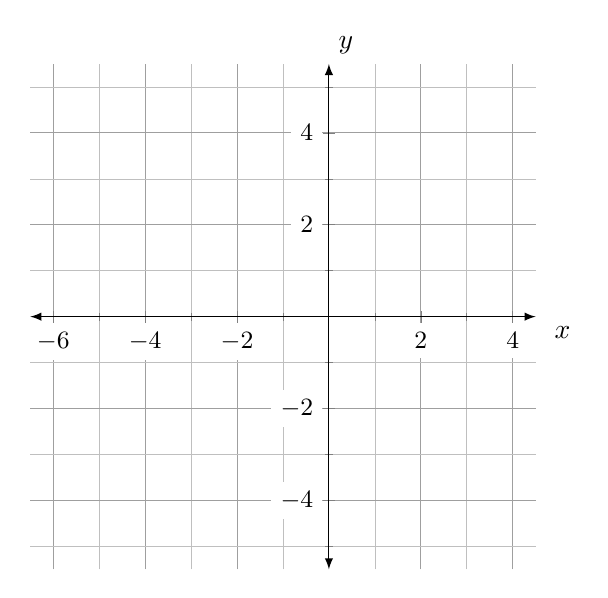
\begin{tikzpicture}[>=latex,scale=1]
				\begin{axis}[
						    width =8cm,
					               height=8cm,
						    xmin=-6,xmax=4,
						    ymin=-5,ymax=5,
						    grid=both,
						    grid style={line width=.2pt, draw=gray!50},
						    major grid style={line width=.3pt,draw=gray!75},
						    axis lines=middle,
						    minor tick num=1,
						    enlargelimits={abs=0.5},
						    axis line style={latex-latex},
						    ticklabel style={font=\small,fill=white},
						    xlabel={\,\,$x$},
						    ylabel={$y$},
						    xlabel style={below right},
						    ylabel style={above right},
						]
				\end{axis}
				%\draw[color=blue,thick] plot (\x,\x*\x);
		\end{tikzpicture}
	\end{center}
\end{minipage}
\hfill
%%%% #8
\begin{minipage}[t]{0.45\linewidth}
\small
	\begin{minipage}[t]{0.45\linewidth}
		\underline{Leading Coefficient}: 3\\
		
		\underline{Degree}: 8 \\
		
		\underline{y-intercept}: 0 \\
		
	\end{minipage}
	\begin{minipage}[t]{0.45\linewidth}
		\begin{tabular}[t]{c|c}
			Roots & Multiplicity\\
			\hline
			-7&3\\
			-4&2\\
			 0& 1\\
			 4& 1\\
			 6&1\\
		\end{tabular}
	\end{minipage}
\normalsize
	\vspace{-0.5cm}
	\begin{center}
		 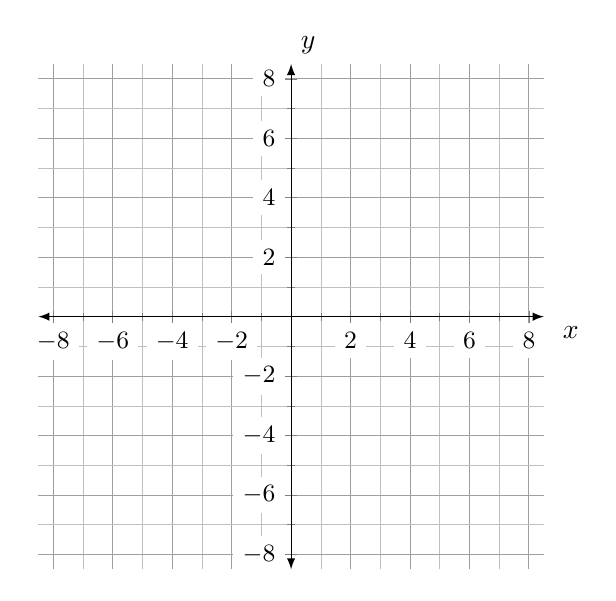
\begin{tikzpicture}[>=latex,scale=1]
				\begin{axis}[
						    width =8cm,
					               height=8cm,
						    xmin=-8,xmax=8,
						    ymin=-8,ymax=8,
						    grid=both,
						    grid style={line width=.2pt, draw=gray!50},
						    major grid style={line width=.3pt,draw=gray!75},
						    axis lines=middle,
						    minor tick num=1,
						    enlargelimits={abs=0.5},
						    axis line style={latex-latex},
						    ticklabel style={font=\small,fill=white},
						    xlabel={\,\,$x$},
						    ylabel={$y$},
						    xlabel style={below right},
						    ylabel style={above right},
						]
				\end{axis}
				%\draw[color=blue,thick] plot (\x,\x*\x);
		\end{tikzpicture}
	\end{center}
\end{minipage}
%%%%%%%%%%%%NEW LINE%%%%%%%%%%%%%%%%%%%%%%%%%
\vfill

%%%%%%%%%%%%%%%%%%%%%%%%%%%%%%%%%%%%%
%%%%%%%%%%%%%%%%%%%%%%%%%%%%%%%%%%%%%
 \newpage
%%%%%%%%%%%%%%%%%%%%%%%%%%%%%%%%%%%%%
%%%%%%%%%%%%%%%%%%%%%%%%%%%%%%%%%%%%%

%%%%%%%%%%%%%%%%%%%%%%%%%%%%%%%
%%%%%%%%%%%%%%%%%%%%%%%%%%%%%%%
%%%%%%   Chapter 6 Review   %%%%%%%%
%%%%%%%%%%%%%%%%%%%%%%%%%%%%%%%
%%%%%%%%%%%%%%%%%%%%%%%%%%%%%%%
\rhead{Algebra 2: Chapter \getcurrentref{chapter} Review} 
\hspace{-1.6cm} \noindent\Large\textbf{Chapter 6 Review (day 1)}\large
 %%%%%%%%%%%%%%%%%%%%%%%%%%%%%%%%
 %%%%%%%%%%%%%%%%%%%%%%%%%%%%%%%%

\begin{enumerate}
\hspace{-2cm} Determine whether the givien binomail is a factor of the polynomial $P(x)$. Use synthetic division.\\

	\begin{minipage}[t]{0.45\linewidth}
		\item $(x+3); P(x)=x^3+2x^2-5$
	\end{minipage}
	\hfill
	\begin{minipage}[t]{0.45\linewidth}
		\item $(x-2); P(x)=2x^3-3x^2+x-6$
	\end{minipage}
	\vspace{3cm}
	
\hspace{-2cm}  Factor each expression.\\

	\begin{minipage}[t]{0.45\linewidth}
		\item  $x^3-x^2-16x+16$
	\end{minipage}
	\hfill
	\begin{minipage}[t]{0.45\linewidth}
		\item $4x^3-8x^2-x+2$
	\end{minipage}
	\vspace{3cm}
	
\hspace{-2cm}  Identify all of the real roots of each equation. Use the Rational Root Theorem and synthetic division.\\

	\begin{minipage}[t]{0.45\linewidth}
		\item $x^3-5x^2+8x-4=0$
	\end{minipage}
	\hfill
	\begin{minipage}[t]{0.45\linewidth}
		\item $x^3+6x^2+9x+2=0$
	\end{minipage}
	
	\vspace{4cm}
	
	\begin{minipage}[t]{0.45\linewidth}
		\item $x^3+3x^2+3x+1=0$
	\end{minipage}
	\hfill
	\begin{minipage}[t]{0.45\linewidth}
		\item $x^4-12x^2+27=0$
	\end{minipage}
	
	\vspace{4cm}
	
	\begin{minipage}[t]{0.45\linewidth}
		\item $x^3+x^2-2x-2=0$
	\end{minipage}
	\hfill
	\begin{minipage}[t]{0.45\linewidth}
		\item $x^3-5x^2+4=0$
	\end{minipage}




\vfill

%%%%%%%%%%%%%%%%%%%%%%%%%%%%%%%%%%%%%
%%%%%%%%%%%%%%%%%%%%%%%%%%%%%%%%%%%%%
 \newpage
%%%%%%%%%%%%%%%%%%%%%%%%%%%%%%%%%%%%%
%%%%%%%%%%%%%%%%%%%%%%%%%%%%%%%%%%%%%

\hspace{-2cm} Write the simplest polynomial function with the given roots.

	\begin{minipage}[t]{0.45\linewidth}
		\item $-3, 2, 4$
	\end{minipage}
	\hfill
	\begin{minipage}[t]{0.45\linewidth}
		\item $-\sqrt{2},-1$
	\end{minipage}
	
	\vspace{4cm}
	
	\begin{minipage}[t]{0.45\linewidth}
		\item $-3, i$
	\end{minipage}
	\hfill
	\begin{minipage}[t]{0.45\linewidth}
		\item $0,1,2i$
	\end{minipage}
	
		\vspace{4cm}
	
\hspace{-2cm} Solve the equation by finding all roots.
	
	\begin{minipage}[t]{0.45\linewidth}
		\item $x^3-x^2+4x-4=0$
	\end{minipage}
	\hfill
	\begin{minipage}[t]{0.45\linewidth}
		\item $x^4-x^2-2=0$
	\end{minipage}
	
		\vspace{4cm}
	
	
\hspace{-2cm}  Identify the leading coefficent, degree and end behavior.
	
	\begin{minipage}[t]{0.45\linewidth}
		\item $-x^3+5x^2+3$\\
		
		\vspace{0.5cm}
		\underline{Degree:}\\
		
		\vspace{0.5cm}
		\underline{Leading Coefficient:}\\

		\vspace{0.5cm}
		\underline{End Behavior:}
	\end{minipage}
	\hfill
	\begin{minipage}[t]{0.45\linewidth}
		\item $-x^6+9x^3-2x-9$\\
		
		\vspace{0.5cm}
		\underline{Degree:}\\
		
		\vspace{0.5cm}
		\underline{Leading Coefficient:}\\
		
		\vspace{0.5cm}
		\underline{End Behavior:}
	\end{minipage}


	
\vspace{2cm}


%%%%%%%%%%%%%%%%%%%%%%%%%%%%%%%%%%%%%
%%%%%%%%%%%%%%%%%%%%%%%%%%%%%%%%%%%%%
 \newpage
%%%%%%%%%%%%%%%%%%%%%%%%%%%%%%%%%%%%%
%%%%%%%%%%%%%%%%%%%%%%%%%%%%%%%%%%%%%


\hspace{-2cm}\noindent Sketch the polynomial function with the given properties. \hfill \textbf{Ch 6 Review (day 2)}\\ \normalsize


%%%%% #19
\begin{minipage}[t]{0.45\linewidth}
\item
\small
	\begin{minipage}[t]{0.45\linewidth}
		\underline{Leading Coefficient}: -1\\
		
		\underline{Degree}: 5 \\
		
		\underline{y-intercept}: 3 \\
		
	\end{minipage}
	\begin{minipage}[t]{0.45\linewidth}
		\begin{tabular}[t]{c|c}
			Roots & Multiplicity\\
			\hline
			-5&2\\
			-2&2\\
			1&1\\

		\end{tabular}
	\end{minipage}
\normalsize
	\vspace{-0.5cm}
	\begin{center}
		 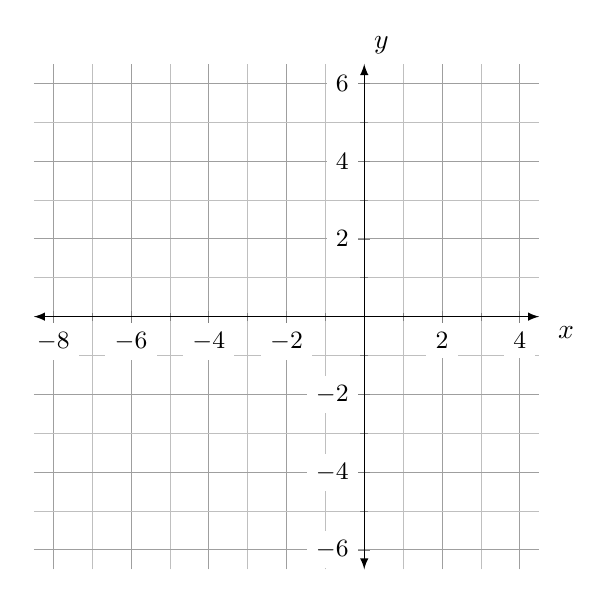
\begin{tikzpicture}[>=latex,scale=1]
				\begin{axis}[
						    width =8cm,
					               height=8cm,
						    xmin=-8,xmax=4,
						    ymin=-6,ymax=6,
						    grid=both,
						    grid style={line width=.2pt, draw=gray!50},
						    major grid style={line width=.3pt,draw=gray!75},
						    axis lines=middle,
						    minor tick num=1,
						    enlargelimits={abs=0.5},
						    axis line style={latex-latex},
						    ticklabel style={font=\small,fill=white},
						    xlabel={\,\,$x$},
						    ylabel={$y$},
						    xlabel style={below right},
						    ylabel style={above right},
						]
				\end{axis}
				%\draw[color=blue,thick] plot (\x,\x*\x);
		\end{tikzpicture}
	\end{center}
\end{minipage}
\hfill
%%%%% #20
\begin{minipage}[t]{0.45\linewidth}
\item
\small
	\begin{minipage}[t]{0.45\linewidth}
		\underline{Leading Coefficient}: 3\\
		
		\underline{Degree}: 8 \\
		
		\underline{y-intercept}: 1 \\
		
	\end{minipage}
	\begin{minipage}[t]{0.45\linewidth}
		\begin{tabular}[t]{c|c}
			Roots & Multiplicity\\
			\hline
			-3&3\\
			-1&3\\
			2&2\\
		\end{tabular}
	\end{minipage}
\normalsize
	\vspace{-0.5cm}
	\begin{center}
		 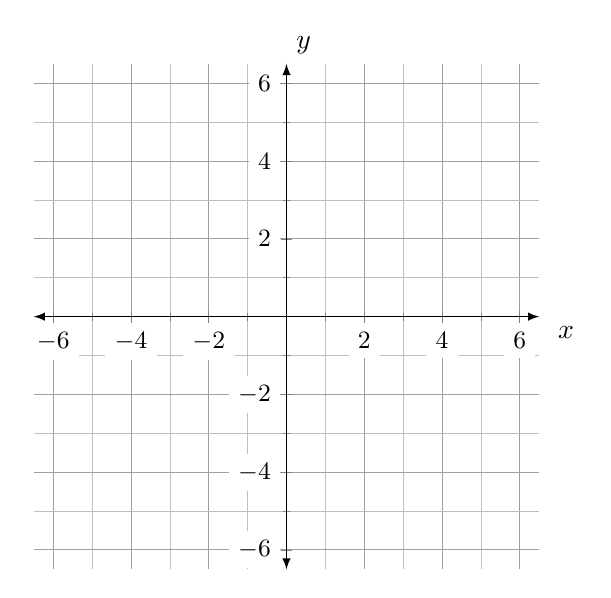
\begin{tikzpicture}[>=latex,scale=1]
				\begin{axis}[
						    width =8cm,
					               height=8cm,
						    xmin=-6,xmax=6,
						    ymin=-6,ymax=6,
						    grid=both,
						    grid style={line width=.2pt, draw=gray!50},
						    major grid style={line width=.3pt,draw=gray!75},
						    axis lines=middle,
						    minor tick num=1,
						    enlargelimits={abs=0.5},
						    axis line style={latex-latex},
						    ticklabel style={font=\small,fill=white},
						    xlabel={\,\,$x$},
						    ylabel={$y$},
						    xlabel style={below right},
						    ylabel style={above right},
						]
				\end{axis}
				%\draw[color=blue,thick] plot (\x,\x*\x);
		\end{tikzpicture}
	\end{center}
\end{minipage}
%%%%%%%%%%%%%%%NEW LINE%%%%%%%%%%%%%%%%%%%%%%
\vfill

%%%%% # 21
\begin{minipage}[t]{0.45\linewidth}
\item
\small
	\begin{minipage}[t]{0.45\linewidth}
		\underline{Leading Coefficient}: 2\\
		
		\underline{Degree}: 3 \\
		
		\underline{y-intercept}: 2 \\
		
	\end{minipage}
	\begin{minipage}[t]{0.45\linewidth}
		\begin{tabular}[t]{c|c}
			Roots & Multiplicity\\
			\hline
			-2&1\\
		\end{tabular}
	\end{minipage}
\normalsize
	\vspace{-0.5cm}
	\begin{center}
		 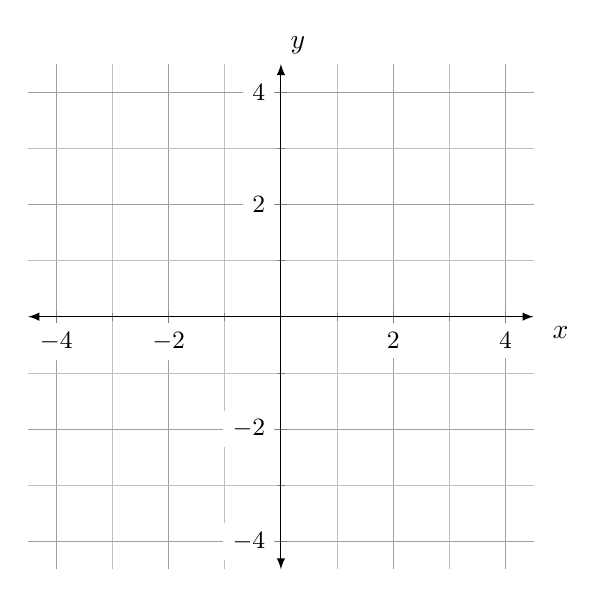
\begin{tikzpicture}[>=latex,scale=1]
				\begin{axis}[
						    width =8cm,
					               height=8cm,
						    xmin=-4,xmax=4,
						    ymin=-4,ymax=4,
						    grid=both,
						    grid style={line width=.2pt, draw=gray!50},
						    major grid style={line width=.3pt,draw=gray!75},
						    axis lines=middle,
						    minor tick num=1,
						    enlargelimits={abs=0.5},
						    axis line style={latex-latex},
						    ticklabel style={font=\small,fill=white},
						    xlabel={\,\,$x$},
						    ylabel={$y$},
						    xlabel style={below right},
						    ylabel style={above right},
						]
				\end{axis}
				%\draw[color=blue,thick] plot (\x,\x*\x);
		\end{tikzpicture}
	\end{center}
\end{minipage}
\hfill
%%%% #22
\begin{minipage}[t]{0.45\linewidth}
\item
\small
	\begin{minipage}[t]{0.45\linewidth}
		\underline{Leading Coefficient}: -1 \\
		
		\underline{Degree}: 2 \\
		
		\underline{y-intercept}: 4 \\
		
	\end{minipage}
	\begin{minipage}[t]{0.45\linewidth}
		\begin{tabular}[t]{c|c}
			Roots & Multiplicity\\
			\hline
			2&1\\
			-2&1\\

		\end{tabular}
	\end{minipage}
\normalsize
	\vspace{-0.5cm}
	\begin{center}
		 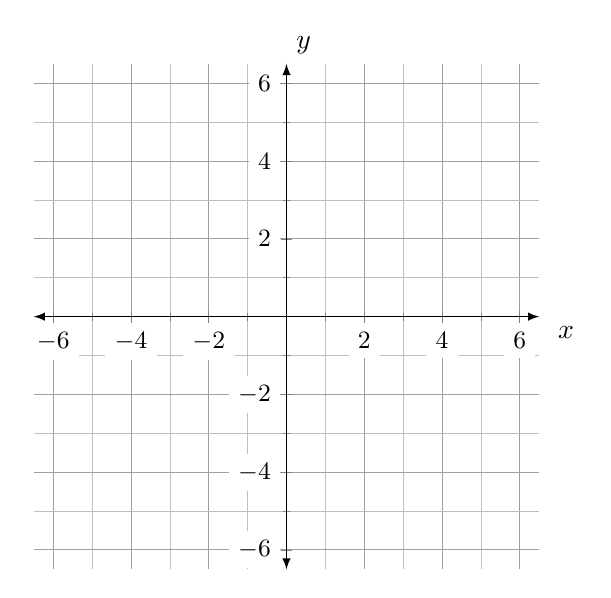
\begin{tikzpicture}[>=latex,scale=1]
				\begin{axis}[
						    width =8cm,
					               height=8cm,
						    xmin=-6,xmax=6,
						    ymin=-6,ymax=6,
						    grid=both,
						    grid style={line width=.2pt, draw=gray!50},
						    major grid style={line width=.3pt,draw=gray!75},
						    axis lines=middle,
						    minor tick num=1,
						    enlargelimits={abs=0.5},
						    axis line style={latex-latex},
						    ticklabel style={font=\small,fill=white},
						    xlabel={\,\,$x$},
						    ylabel={$y$},
						    xlabel style={below right},
						    ylabel style={above right},
						]
				\end{axis}
				%\draw[color=blue,thick] plot (\x,\x*\x);
		\end{tikzpicture}
	\end{center}
\end{minipage}

\vfill

%%%%%%%%%%%%%%%%%%%%%%%%%%%%%%%%%%%%%
%%%%%%%%%%%%%%%%%%%%%%%%%%%%%%%%%%%%%
 \newpage
%%%%%%%%%%%%%%%%%%%%%%%%%%%%%%%%%%%%%
%%%%%%%%%%%%%%%%%%%%%%%%%%%%%%%%%%%%%



\hspace{-2cm}\large \noindent Sketch the polynomial function.\\\normalsize 


%%%%% #23
\begin{minipage}[t]{0.45\linewidth}
\item
\small
	\begin{minipage}[t]{\linewidth}
		$P(x)=(x+4)^2(x+1)^2(x-1)$
	\end{minipage}
\normalsize
	\vspace{-0.5cm}
	\begin{center}
		 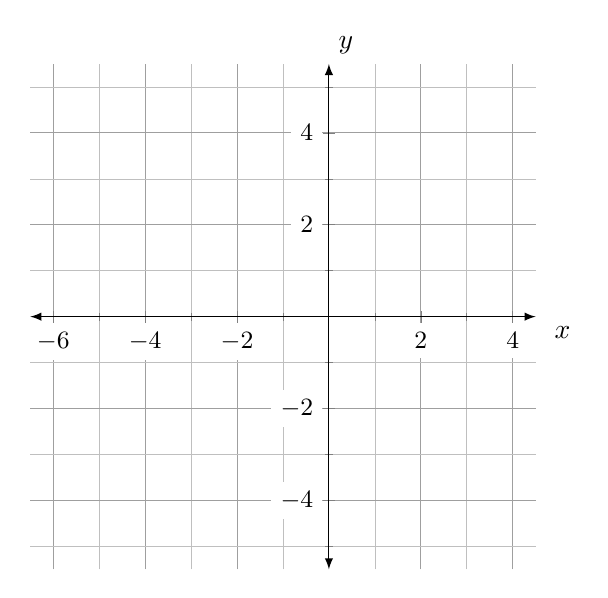
\begin{tikzpicture}[>=latex,scale=1]
				\begin{axis}[
						    width =8cm,
					               height=8cm,
						    xmin=-6,xmax=4,
						    ymin=-5,ymax=5,
						    grid=both,
						    grid style={line width=.2pt, draw=gray!50},
						    major grid style={line width=.3pt,draw=gray!75},
						    axis lines=middle,
						    minor tick num=1,
						    enlargelimits={abs=0.5},
						    axis line style={latex-latex},
						    ticklabel style={font=\small,fill=white},
						    xlabel={\,\,$x$},
						    ylabel={$y$},
						    xlabel style={below right},
						    ylabel style={above right},
						]
				\end{axis}
				%\draw[color=blue,thick] plot (\x,\x*\x);
		\end{tikzpicture}
	\end{center}
\end{minipage}
\hfill
%%%%% #24
\begin{minipage}[t]{0.45\linewidth}
\item
\small
	\begin{minipage}[t]{\linewidth}
		$f(x)=(x+5)(x+1)(x-3)$
		
	\end{minipage}
\normalsize
	\vspace{-0.5cm}
	\begin{center}
		 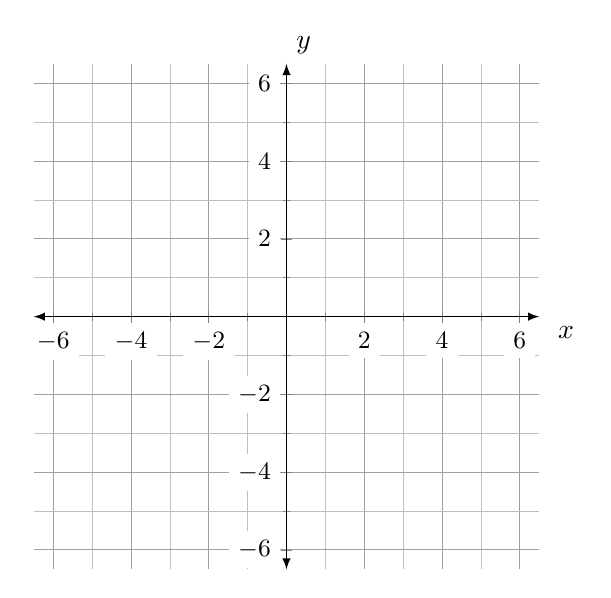
\begin{tikzpicture}[>=latex,scale=1]
				\begin{axis}[
						    width =8cm,
					               height=8cm,
						    xmin=-6,xmax=6,
						    ymin=-6,ymax=6,
						    grid=both,
						    grid style={line width=.2pt, draw=gray!50},
						    major grid style={line width=.3pt,draw=gray!75},
						    axis lines=middle,
						    minor tick num=1,
						    enlargelimits={abs=0.5},
						    axis line style={latex-latex},
						    ticklabel style={font=\small,fill=white},
						    xlabel={\,\,$x$},
						    ylabel={$y$},
						    xlabel style={below right},
						    ylabel style={above right},
						]
				\end{axis}
				%\draw[color=blue,thick] plot (\x,\x*\x);
		\end{tikzpicture}
	\end{center}
\end{minipage}
%%%%%%%%%%%%%%%NEW LINE%%%%%%%%%%%%%%%%%%%%%%
\vfill


%%%%% #25
\begin{minipage}[t]{0.45\linewidth}
\item
\small
	\begin{minipage}[t]{\linewidth}
		$P(x)=-2(x+6)^3(x+3)^2(x-2)^2$
	\end{minipage}
\normalsize
	\vspace{-0.5cm}
	\begin{center}
		 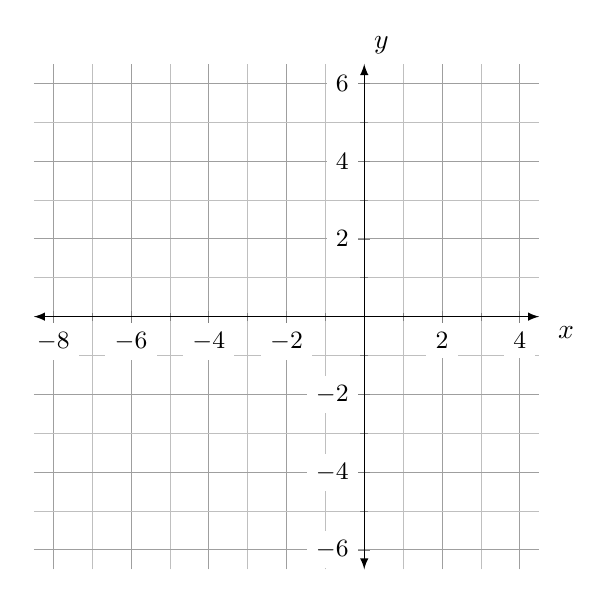
\begin{tikzpicture}[>=latex,scale=1]
				\begin{axis}[
						    width =8cm,
					               height=8cm,
						    xmin=-8,xmax=4,
						    ymin=-6,ymax=6,
						    grid=both,
						    grid style={line width=.2pt, draw=gray!50},
						    major grid style={line width=.3pt,draw=gray!75},
						    axis lines=middle,
						    minor tick num=1,
						    enlargelimits={abs=0.5},
						    axis line style={latex-latex},
						    ticklabel style={font=\small,fill=white},
						    xlabel={\,\,$x$},
						    ylabel={$y$},
						    xlabel style={below right},
						    ylabel style={above right},
						]
				\end{axis}
				%\draw[color=blue,thick] plot (\x,\x*\x);
		\end{tikzpicture}
	\end{center}
\end{minipage}
\hfill
%%%%% #26
\begin{minipage}[t]{0.45\linewidth}
\item
\small
	\begin{minipage}[t]{\linewidth}
		$f(x)=-3x^4(x+3)^2(x-3)^3$
		
	\end{minipage}
\normalsize
	\vspace{-0.5cm}
	\begin{center}
		 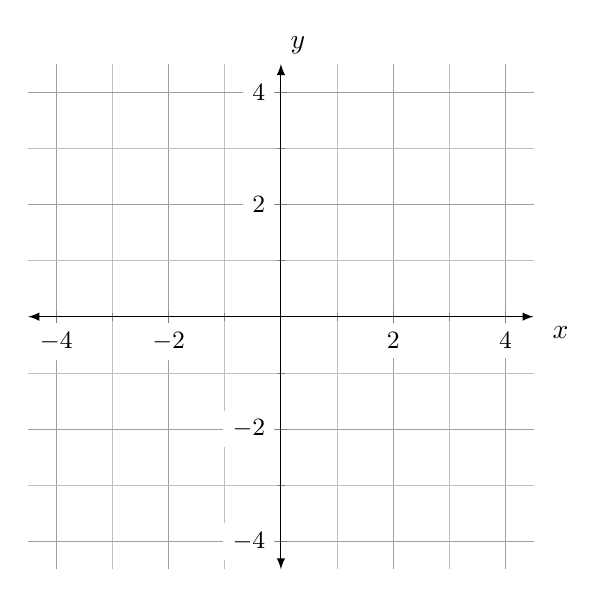
\begin{tikzpicture}[>=latex,scale=1]
				\begin{axis}[
						    width =8cm,
					               height=8cm,
						    xmin=-4,xmax=4,
						    ymin=-4,ymax=4,
						    grid=both,
						    grid style={line width=.2pt, draw=gray!50},
						    major grid style={line width=.3pt,draw=gray!75},
						    axis lines=middle,
						    minor tick num=1,
						    enlargelimits={abs=0.5},
						    axis line style={latex-latex},
						    ticklabel style={font=\small,fill=white},
						    xlabel={\,\,$x$},
						    ylabel={$y$},
						    xlabel style={below right},
						    ylabel style={above right},
						]
				\end{axis}
				%\draw[color=blue,thick] plot (\x,\x*\x);
		\end{tikzpicture}
	\end{center}
\end{minipage}


%%%%% #27
\begin{minipage}[t]{0.45\linewidth}
\item
\small
	\begin{minipage}[t]{\linewidth}
		$H(x)=x^3-4x^2-7x+10$
	\end{minipage}
\normalsize
	\vspace{-0.5cm}
	\begin{center}
		 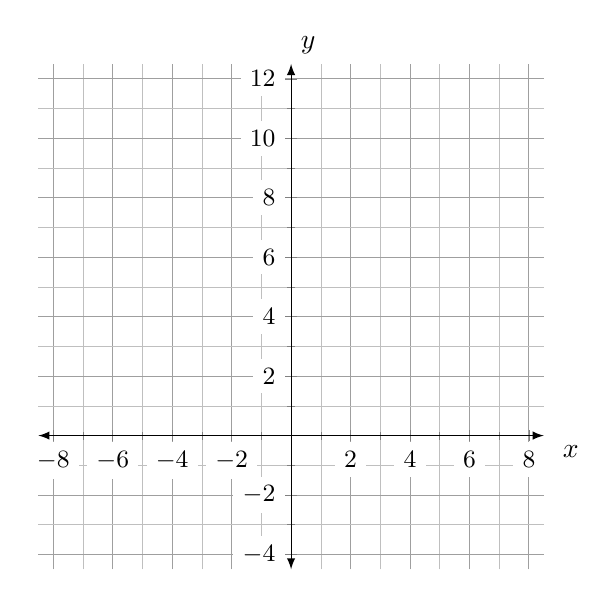
\begin{tikzpicture}[>=latex,scale=1]
				\begin{axis}[
						    width =8cm,
					               height=8cm,
						    xmin=-8,xmax=8,
						    ymin=-4,ymax=12,
						    grid=both,
						    grid style={line width=.2pt, draw=gray!50},
						    major grid style={line width=.3pt,draw=gray!75},
						    axis lines=middle,
						    minor tick num=1,
						    enlargelimits={abs=0.5},
						    axis line style={latex-latex},
						    ticklabel style={font=\small,fill=white},
						    xlabel={\,\,$x$},
						    ylabel={$y$},
						    xlabel style={below right},
						    ylabel style={above right},
						]
				\end{axis}
				%\draw[color=blue,thick] plot (\x,\x*\x);
		\end{tikzpicture}
	\end{center}
\end{minipage}
\hfill
%%%% #28
\begin{minipage}[t]{0.45\linewidth}
\item
\small
	\begin{minipage}[t]{0.45\linewidth}
		$Q(x)=x^3+x^2-9x-9$
	\end{minipage}
\normalsize
	\begin{center}
		 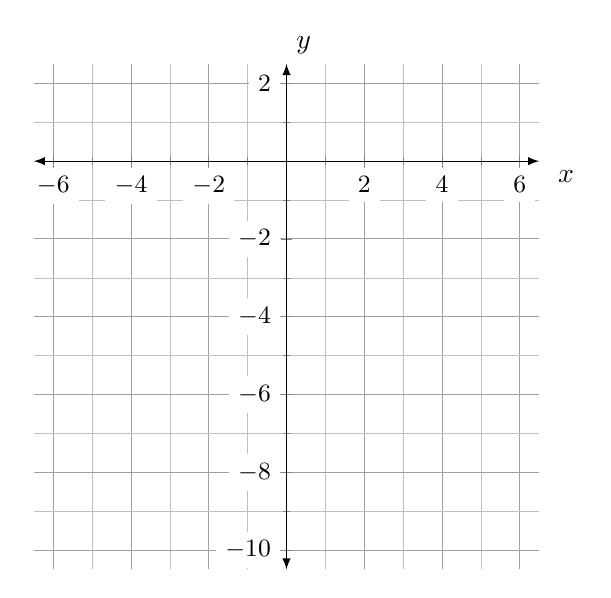
\begin{tikzpicture}[>=latex,scale=1]
				\begin{axis}[
						    width =8cm,
					               height=8cm,
						    xmin=-6,xmax=6,
						    ymin=-10,ymax=2,
						    grid=both,
						    grid style={line width=.2pt, draw=gray!50},
						    major grid style={line width=.3pt,draw=gray!75},
						    axis lines=middle,
						    minor tick num=1,
						    enlargelimits={abs=0.5},
						    axis line style={latex-latex},
						    ticklabel style={font=\small,fill=white},
						    xlabel={\,\,$x$},
						    ylabel={$y$},
						    xlabel style={below right},
						    ylabel style={above right},
						]
				\end{axis}
				%\draw[color=blue,thick] plot (\x,\x*\x);
		\end{tikzpicture}
	\end{center}
\end{minipage}

\end{enumerate}

\end{document}










